\documentclass[twoside]{book}

% Packages required by doxygen
\usepackage{calc}
\usepackage{doxygen}
\usepackage{graphicx}
\usepackage[utf8]{inputenc}
\usepackage{makeidx}
\usepackage{multicol}
\usepackage{multirow}
\usepackage{textcomp}
\usepackage[table]{xcolor}

% NLS support packages
\usepackage{polski}
\usepackage[T1]{fontenc}

% Font selection
\usepackage[T1]{fontenc}
\usepackage{mathptmx}
\usepackage[scaled=.90]{helvet}
\usepackage{courier}
\usepackage{amssymb}
\usepackage{sectsty}
\renewcommand{\familydefault}{\sfdefault}
\allsectionsfont{%
  \fontseries{bc}\selectfont%
  \color{darkgray}%
}
\renewcommand{\DoxyLabelFont}{%
  \fontseries{bc}\selectfont%
  \color{darkgray}%
}

% Page & text layout
\usepackage{geometry}
\geometry{%
  a4paper,%
  top=2.5cm,%
  bottom=2.5cm,%
  left=2.5cm,%
  right=2.5cm%
}
\tolerance=750
\hfuzz=15pt
\hbadness=750
\setlength{\emergencystretch}{15pt}
\setlength{\parindent}{0cm}
\setlength{\parskip}{0.2cm}
\makeatletter
\renewcommand{\paragraph}{%
  \@startsection{paragraph}{4}{0ex}{-1.0ex}{1.0ex}{%
    \normalfont\normalsize\bfseries\SS@parafont%
  }%
}
\renewcommand{\subparagraph}{%
  \@startsection{subparagraph}{5}{0ex}{-1.0ex}{1.0ex}{%
    \normalfont\normalsize\bfseries\SS@subparafont%
  }%
}
\makeatother

% Headers & footers
\usepackage{fancyhdr}
\pagestyle{fancyplain}
\fancyhead[LE]{\fancyplain{}{\bfseries\thepage}}
\fancyhead[CE]{\fancyplain{}{}}
\fancyhead[RE]{\fancyplain{}{\bfseries\leftmark}}
\fancyhead[LO]{\fancyplain{}{\bfseries\rightmark}}
\fancyhead[CO]{\fancyplain{}{}}
\fancyhead[RO]{\fancyplain{}{\bfseries\thepage}}
\fancyfoot[LE]{\fancyplain{}{}}
\fancyfoot[CE]{\fancyplain{}{}}
\fancyfoot[RE]{\fancyplain{}{\bfseries\scriptsize Wygenerowano Śr, 25 mar 2015 23\-:23\-:29 dla lab3 programem Doxygen }}
\fancyfoot[LO]{\fancyplain{}{\bfseries\scriptsize Wygenerowano Śr, 25 mar 2015 23\-:23\-:29 dla lab3 programem Doxygen }}
\fancyfoot[CO]{\fancyplain{}{}}
\fancyfoot[RO]{\fancyplain{}{}}
\renewcommand{\footrulewidth}{0.4pt}
\renewcommand{\chaptermark}[1]{%
  \markboth{#1}{}%
}
\renewcommand{\sectionmark}[1]{%
  \markright{\thesection\ #1}%
}

% Indices & bibliography
\usepackage{natbib}
\usepackage[titles]{tocloft}
\setcounter{tocdepth}{3}
\setcounter{secnumdepth}{5}
\makeindex

% Hyperlinks (required, but should be loaded last)
\usepackage{ifpdf}
\ifpdf
  \usepackage[pdftex,pagebackref=true]{hyperref}
\else
  \usepackage[ps2pdf,pagebackref=true]{hyperref}
\fi
\hypersetup{%
  colorlinks=true,%
  linkcolor=blue,%
  citecolor=blue,%
  unicode%
}

% Custom commands
\newcommand{\clearemptydoublepage}{%
  \newpage{\pagestyle{empty}\cleardoublepage}%
}


%===== C O N T E N T S =====

\begin{document}

% Titlepage & ToC
\hypersetup{pageanchor=false}
\pagenumbering{roman}
\begin{titlepage}
\vspace*{7cm}
\begin{center}%
{\Large lab3 \\[1ex]\large 0.\-0003 }\\
\vspace*{1cm}
{\large Wygenerowano przez Doxygen 1.8.6}\\
\vspace*{0.5cm}
{\small Śr, 25 mar 2015 23:23:29}\\
\end{center}
\end{titlepage}
\clearemptydoublepage
\tableofcontents
\clearemptydoublepage
\pagenumbering{arabic}
\hypersetup{pageanchor=true}

%--- Begin generated contents ---
\chapter{Laboratorium 3}
\label{index}\hypertarget{index}{}\begin{DoxyAuthor}{Autor}
Filip Malinowski 
\end{DoxyAuthor}
\begin{DoxyDate}{Data}
22.\-04.\-2015 
\end{DoxyDate}
\begin{DoxyVersion}{Wersja}
0.\-0005
\end{DoxyVersion}
Program sluzacy do uruchamiania algorytmow i badania ich szybkosci dzialania.\par
W programie zaimplementowane sa algorytmy\-:\par

\begin{DoxyItemize}
\item sortowania szybkiego stosu\par

\item sortowania szybkiego po optymalizacji pivot stosu\par

\item sortowania przez scalanie stosu\par

\item sortowania przez kopcowanie stosu
\end{DoxyItemize}

Do wykonania podanych powyzej trzech ostatnich algorytmow zostaly zaimplementowane potrzebne struktury danych (stos, kolejka, lista oraz lista tablicowa, lista asocjacyjna, tablica z haszowaniem).\par
\par
Ciala klas znajduja sie w folderze ./prj/inc\par
Definicje metod znajduja sie w folderze ./prj/src\par
Sprawozdanie znajduje sie w folderze ./prj/doc/sprawozdanie\par
\par
Format wywolania\-:\par

\begin{DoxyCode}
./prj/make clean\(\backslash\)n
./prj/make\(\backslash\)n
\end{DoxyCode}
 
\chapter{Indeks hierarchiczny}
\section{Hierarchia klas}
Ta lista dziedziczenia posortowana jest z grubsza, choć nie całkowicie, alfabetycznie\-:\begin{DoxyCompactList}
\item \contentsline{section}{Benchmark}{\pageref{class_benchmark}}{}
\begin{DoxyCompactList}
\item \contentsline{section}{Mnozenie}{\pageref{class_mnozenie}}{}
\end{DoxyCompactList}
\end{DoxyCompactList}

\chapter{Indeks klas}
\section{Lista klas}
Tutaj znajdują się klasy, struktury, unie i interfejsy wraz z ich krótkimi opisami\-:\begin{DoxyCompactList}
\item\contentsline{section}{\hyperlink{class_algorithm_kolejka}{Algorithm\-Kolejka} \\*Klasa \hyperlink{class_algorithm_kolejka}{Algorithm\-Kolejka} modelujaca algorytm wczytywania do kolejki. Obiekt tego typu reprezentuje algorytm wykonujacy wykonujacy wczytywanie zadanej ilosci elementow do kolejki }{\pageref{class_algorithm_kolejka}}{}
\item\contentsline{section}{\hyperlink{class_algorithm_lista}{Algorithm\-Lista} \\*Klasa \hyperlink{class_algorithm_lista}{Algorithm\-Lista} modelujaca algorytm wczytywania do kolejki. Obiekt tego typu reprezentuje algorytm wykonujacy wykonujacy wczytywanie zadanej ilosci elementow do listy }{\pageref{class_algorithm_lista}}{}
\item\contentsline{section}{\hyperlink{class_algorithm_stos}{Algorithm\-Stos} \\*Klasa \hyperlink{class_algorithm_stos}{Algorithm\-Stos} modelujaca algorytm wczytywania do stosu. Obiekt tego typu reprezentuje algorytm wykonujacy wykonujacy wczytywanie zadanej ilosci elementow do stosu }{\pageref{class_algorithm_stos}}{}
\item\contentsline{section}{\hyperlink{class_benchmark}{Benchmark} \\*Klasa \hyperlink{class_benchmark}{Benchmark} modelujaca program benchmarkujacy. Obiekt tego typu reprezentuje program sprawdzajacy szybkosc wykonywania algorytmow }{\pageref{class_benchmark}}{}
\item\contentsline{section}{\hyperlink{class_kolejka}{Kolejka} \\*Klasa \hyperlink{class_kolejka}{Kolejka} modelujaca strukture danych typu kolejka. Obiekt tego typu reprezentuje strukture danych typu kolejka wraz z operacjami mozliwymi do wykonania na tej strukturze }{\pageref{class_kolejka}}{}
\item\contentsline{section}{\hyperlink{struct_lista_1_1_komorka}{Lista\-::\-Komorka} \\*Struktura \hyperlink{struct_lista_1_1_komorka}{Komorka}. Obiekt tego typu reprezentuje pojedyncza komorke wraz ze wskaznikiem na nastepna komorke listy }{\pageref{struct_lista_1_1_komorka}}{}
\item\contentsline{section}{\hyperlink{class_lista}{Lista} \\*Klasa \hyperlink{class_lista}{Lista} modelujaca strukture danych typu lista. Obiekt tego typu reprezentuje strukture danych typu lista wraz z operacjami mozliwymi do wykonania na tej strukturze }{\pageref{class_lista}}{}
\item\contentsline{section}{\hyperlink{class_mnozenie}{Mnozenie} \\*Klasa \hyperlink{class_mnozenie}{Mnozenie} modelujaca algorytm mnozenia. Obiekt tego typu reprezentuje algorytm wykonujacy dzialanie mnozenia kazdego elementu tablicy tab przez 2 }{\pageref{class_mnozenie}}{}
\item\contentsline{section}{\hyperlink{class_stos}{Stos} \\*Klasa \hyperlink{class_stos}{Stos} modelujaca strukture danych typu stos. Obiekt tego typu reprezentuje strukture danych typu stos wraz z operacjami mozliwymi do wykonania na tej strukturze }{\pageref{class_stos}}{}
\end{DoxyCompactList}

\chapter{Indeks plików}
\section{Lista plików}
Tutaj znajduje się lista wszystkich plików z ich krótkimi opisami\-:\begin{DoxyCompactList}
\item\contentsline{section}{\hyperlink{algorithm2_8cpp}{algorithm2.\-cpp} }{\pageref{algorithm2_8cpp}}{}
\item\contentsline{section}{\hyperlink{algorithm2_8hh}{algorithm2.\-hh} }{\pageref{algorithm2_8hh}}{}
\item\contentsline{section}{\hyperlink{algorithm__kolejka_8cpp}{algorithm\-\_\-kolejka.\-cpp} }{\pageref{algorithm__kolejka_8cpp}}{}
\item\contentsline{section}{\hyperlink{algorithm__kolejka_8hh}{algorithm\-\_\-kolejka.\-hh} }{\pageref{algorithm__kolejka_8hh}}{}
\item\contentsline{section}{\hyperlink{algorithm__lista_8cpp}{algorithm\-\_\-lista.\-cpp} }{\pageref{algorithm__lista_8cpp}}{}
\item\contentsline{section}{\hyperlink{algorithm__lista_8hh}{algorithm\-\_\-lista.\-hh} }{\pageref{algorithm__lista_8hh}}{}
\item\contentsline{section}{\hyperlink{algorithm__stos_8cpp}{algorithm\-\_\-stos.\-cpp} }{\pageref{algorithm__stos_8cpp}}{}
\item\contentsline{section}{\hyperlink{algorithm__stos_8hh}{algorithm\-\_\-stos.\-hh} }{\pageref{algorithm__stos_8hh}}{}
\item\contentsline{section}{\hyperlink{benchmark_8cpp}{benchmark.\-cpp} }{\pageref{benchmark_8cpp}}{}
\item\contentsline{section}{\hyperlink{benchmark_8hh}{benchmark.\-hh} }{\pageref{benchmark_8hh}}{}
\item\contentsline{section}{\hyperlink{generate_8cpp}{generate.\-cpp} }{\pageref{generate_8cpp}}{}
\item\contentsline{section}{\hyperlink{kolejka_8cpp}{kolejka.\-cpp} }{\pageref{kolejka_8cpp}}{}
\item\contentsline{section}{\hyperlink{kolejka_8hh}{kolejka.\-hh} }{\pageref{kolejka_8hh}}{}
\item\contentsline{section}{\hyperlink{lista_8cpp}{lista.\-cpp} }{\pageref{lista_8cpp}}{}
\item\contentsline{section}{\hyperlink{lista_8hh}{lista.\-hh} }{\pageref{lista_8hh}}{}
\item\contentsline{section}{\hyperlink{main_8cpp}{main.\-cpp} }{\pageref{main_8cpp}}{}
\item\contentsline{section}{\hyperlink{stos_8cpp}{stos.\-cpp} }{\pageref{stos_8cpp}}{}
\item\contentsline{section}{\hyperlink{stos_8hh}{stos.\-hh} }{\pageref{stos_8hh}}{}
\item\contentsline{section}{\hyperlink{tab__lista_8cpp}{tab\-\_\-lista.\-cpp} }{\pageref{tab__lista_8cpp}}{}
\item\contentsline{section}{\hyperlink{tab__lista_8hh}{tab\-\_\-lista.\-hh} }{\pageref{tab__lista_8hh}}{}
\end{DoxyCompactList}

\chapter{Dokumentacja klas}
\hypertarget{class_algorithm2}{\section{Dokumentacja klasy Algorithm2}
\label{class_algorithm2}\index{Algorithm2@{Algorithm2}}
}


Klasa \hyperlink{class_algorithm2}{Algorithm2} modelujaca algorytm sortowania stosu. Obiekt tego typu reprezentuje algorytm wykonujacy sortowanie szybkie na elementach stosu. Dziedziczy po klasie \hyperlink{class_benchmark}{Benchmark}.  




{\ttfamily \#include $<$algorithm2.\-hh$>$}



Diagram dziedziczenia dla Algorithm2\nopagebreak
\begin{figure}[H]
\begin{center}
\leavevmode
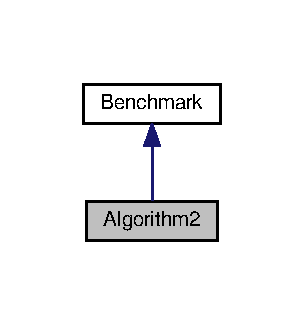
\includegraphics[width=146pt]{class_algorithm2__inherit__graph}
\end{center}
\end{figure}


Diagram współpracy dla Algorithm2\-:\nopagebreak
\begin{figure}[H]
\begin{center}
\leavevmode
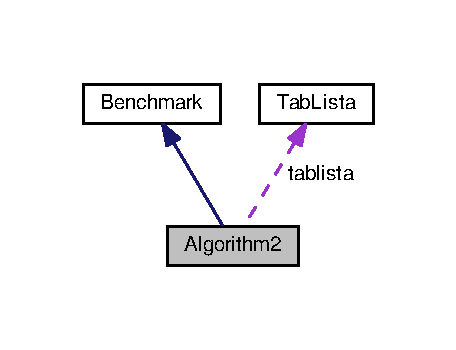
\includegraphics[width=259pt]{class_algorithm2__coll__graph}
\end{center}
\end{figure}
\subsection*{Metody publiczne}
\begin{DoxyCompactItemize}
\item 
\hyperlink{class_algorithm2_ad77a51433815456eca8139444e78b49b}{Algorithm2} ()
\begin{DoxyCompactList}\small\item\em Konstruktor obiektu \hyperlink{class_algorithm2}{Algorithm2}. \end{DoxyCompactList}\item 
\hyperlink{class_algorithm2_a63a761a11070a07905229137034b3cb9}{Algorithm2} (unsigned short $\ast$\-\_\-tab, int \-\_\-id)
\begin{DoxyCompactList}\small\item\em Konstruktor parametryczny obiektu \hyperlink{class_algorithm2}{Algorithm2}. \end{DoxyCompactList}\item 
\hyperlink{class_algorithm2_ab2c630f56f5d2e90f62a13fdaf0cd954}{$\sim$\-Algorithm2} ()
\begin{DoxyCompactList}\small\item\em Destruktor obiektu \hyperlink{class_algorithm2}{Algorithm2}. \end{DoxyCompactList}\item 
virtual void \hyperlink{class_algorithm2_a50bbb4421660c4200dba66e9da9d7969}{load} (int \-\_\-border)
\begin{DoxyCompactList}\small\item\em Metoda przygotowywania algorytmu. Metoda sluzy do przygotowania warunkow do przeprowadzenia testu. \end{DoxyCompactList}\item 
virtual void \hyperlink{class_algorithm2_a3d7e4d0c9308d0b97250cb5596a73165}{unload} (int \-\_\-border)
\begin{DoxyCompactList}\small\item\em Metoda sprzatania. Metoda sluzy do oproznienia struktury. \end{DoxyCompactList}\item 
virtual void \hyperlink{class_algorithm2_a409e58d5fb0b6d2407cc986cf163703b}{run\-Algorithm} (int \-\_\-border)
\begin{DoxyCompactList}\small\item\em Metoda uruchamiania algorytmu. Metoda sluzy do wykonywania danego algorytmu. Sortuje elementy stosu. \end{DoxyCompactList}\end{DoxyCompactItemize}
\subsection*{Atrybuty prywatne}
\begin{DoxyCompactItemize}
\item 
\hyperlink{struct_binary_tree}{Binary\-Tree} \hyperlink{class_algorithm2_aff7c12a2dc0294d120a36ae0efc4af6a}{tree}
\begin{DoxyCompactList}\small\item\em Zmienna przechowujaca drzewo binarne. \end{DoxyCompactList}\end{DoxyCompactItemize}
\subsection*{Dodatkowe Dziedziczone Składowe}


\subsection{Opis szczegółowy}


Definicja w linii 10 pliku algorithm2.\-hh.



\subsection{Dokumentacja konstruktora i destruktora}
\hypertarget{class_algorithm2_ad77a51433815456eca8139444e78b49b}{\index{Algorithm2@{Algorithm2}!Algorithm2@{Algorithm2}}
\index{Algorithm2@{Algorithm2}!Algorithm2@{Algorithm2}}
\subsubsection[{Algorithm2}]{\setlength{\rightskip}{0pt plus 5cm}Algorithm2\-::\-Algorithm2 (
\begin{DoxyParamCaption}
{}
\end{DoxyParamCaption}
)\hspace{0.3cm}{\ttfamily [inline]}}}\label{class_algorithm2_ad77a51433815456eca8139444e78b49b}


Definicja w linii 20 pliku algorithm2.\-hh.

\hypertarget{class_algorithm2_a63a761a11070a07905229137034b3cb9}{\index{Algorithm2@{Algorithm2}!Algorithm2@{Algorithm2}}
\index{Algorithm2@{Algorithm2}!Algorithm2@{Algorithm2}}
\subsubsection[{Algorithm2}]{\setlength{\rightskip}{0pt plus 5cm}Algorithm2\-::\-Algorithm2 (
\begin{DoxyParamCaption}
\item[{unsigned short $\ast$}]{\-\_\-tab, }
\item[{int}]{\-\_\-id}
\end{DoxyParamCaption}
)}}\label{class_algorithm2_a63a761a11070a07905229137034b3cb9}

\begin{DoxyParams}[1]{Parametry}
\mbox{\tt in}  & {\em \-\_\-tab} & -\/ tablica przechowujaca dane wejsciowe. \\
\hline
\mbox{\tt in}  & {\em \-\_\-id} & -\/ identyfikator algorytmu. \\
\hline
\end{DoxyParams}


Definicja w linii 10 pliku algorithm2.\-cpp.

\hypertarget{class_algorithm2_ab2c630f56f5d2e90f62a13fdaf0cd954}{\index{Algorithm2@{Algorithm2}!$\sim$\-Algorithm2@{$\sim$\-Algorithm2}}
\index{$\sim$\-Algorithm2@{$\sim$\-Algorithm2}!Algorithm2@{Algorithm2}}
\subsubsection[{$\sim$\-Algorithm2}]{\setlength{\rightskip}{0pt plus 5cm}Algorithm2\-::$\sim$\-Algorithm2 (
\begin{DoxyParamCaption}
{}
\end{DoxyParamCaption}
)}}\label{class_algorithm2_ab2c630f56f5d2e90f62a13fdaf0cd954}


Definicja w linii 17 pliku algorithm2.\-cpp.



\subsection{Dokumentacja funkcji składowych}
\hypertarget{class_algorithm2_a50bbb4421660c4200dba66e9da9d7969}{\index{Algorithm2@{Algorithm2}!load@{load}}
\index{load@{load}!Algorithm2@{Algorithm2}}
\subsubsection[{load}]{\setlength{\rightskip}{0pt plus 5cm}void Algorithm2\-::load (
\begin{DoxyParamCaption}
\item[{int}]{\-\_\-border}
\end{DoxyParamCaption}
)\hspace{0.3cm}{\ttfamily [virtual]}}}\label{class_algorithm2_a50bbb4421660c4200dba66e9da9d7969}

\begin{DoxyParams}[1]{Parametry}
\mbox{\tt in}  & {\em \-\_\-border} & -\/ ilosc elementow dla ktorych metoda ma wykonac swoje dzialanie. \\
\hline
\end{DoxyParams}


Implementuje \hyperlink{class_benchmark_a41f66d36949f1488facb8e3d49c99f67}{Benchmark}.



Definicja w linii 28 pliku algorithm2.\-cpp.



Oto graf wywołań dla tej funkcji\-:\nopagebreak
\begin{figure}[H]
\begin{center}
\leavevmode
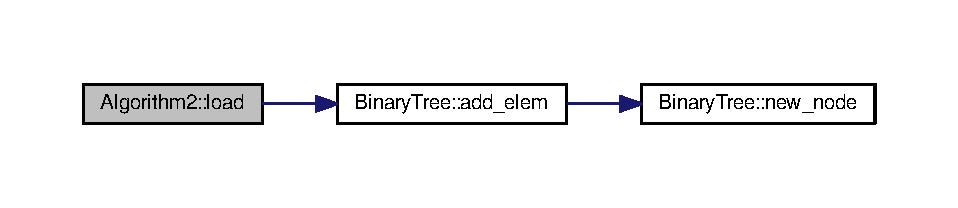
\includegraphics[width=350pt]{class_algorithm2_a50bbb4421660c4200dba66e9da9d7969_cgraph}
\end{center}
\end{figure}


\hypertarget{class_algorithm2_a409e58d5fb0b6d2407cc986cf163703b}{\index{Algorithm2@{Algorithm2}!run\-Algorithm@{run\-Algorithm}}
\index{run\-Algorithm@{run\-Algorithm}!Algorithm2@{Algorithm2}}
\subsubsection[{run\-Algorithm}]{\setlength{\rightskip}{0pt plus 5cm}void Algorithm2\-::run\-Algorithm (
\begin{DoxyParamCaption}
\item[{int}]{\-\_\-border}
\end{DoxyParamCaption}
)\hspace{0.3cm}{\ttfamily [virtual]}}}\label{class_algorithm2_a409e58d5fb0b6d2407cc986cf163703b}

\begin{DoxyParams}[1]{Parametry}
\mbox{\tt in}  & {\em \-\_\-border} & -\/ ilosc elementow dla ktorych algorytm ma wykonac swoje dzialanie. \\
\hline
\end{DoxyParams}


Implementuje \hyperlink{class_benchmark_a33e60395b1e126ca65c3aea3abf6debf}{Benchmark}.



Definicja w linii 22 pliku algorithm2.\-cpp.



Oto graf wywołań dla tej funkcji\-:\nopagebreak
\begin{figure}[H]
\begin{center}
\leavevmode
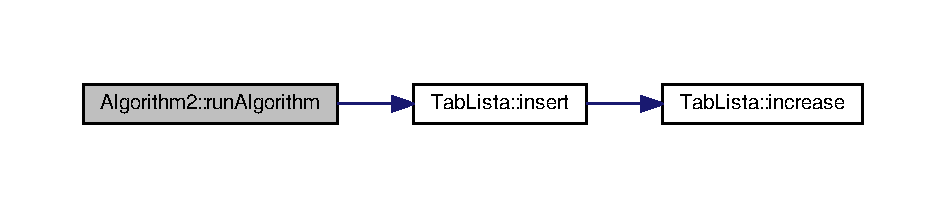
\includegraphics[width=350pt]{class_algorithm2_a409e58d5fb0b6d2407cc986cf163703b_cgraph}
\end{center}
\end{figure}


\hypertarget{class_algorithm2_a3d7e4d0c9308d0b97250cb5596a73165}{\index{Algorithm2@{Algorithm2}!unload@{unload}}
\index{unload@{unload}!Algorithm2@{Algorithm2}}
\subsubsection[{unload}]{\setlength{\rightskip}{0pt plus 5cm}void Algorithm2\-::unload (
\begin{DoxyParamCaption}
\item[{int}]{\-\_\-border}
\end{DoxyParamCaption}
)\hspace{0.3cm}{\ttfamily [virtual]}}}\label{class_algorithm2_a3d7e4d0c9308d0b97250cb5596a73165}

\begin{DoxyParams}[1]{Parametry}
\mbox{\tt in}  & {\em \-\_\-border} & -\/ ilosc elementow dla ktorych metoda ma wykonac swoje dzialanie. \\
\hline
\end{DoxyParams}


Implementuje \hyperlink{class_benchmark_a2dcfb6ee9e648ae88d8c131b2b191bed}{Benchmark}.



Definicja w linii 35 pliku algorithm2.\-cpp.



Oto graf wywołań dla tej funkcji\-:\nopagebreak
\begin{figure}[H]
\begin{center}
\leavevmode
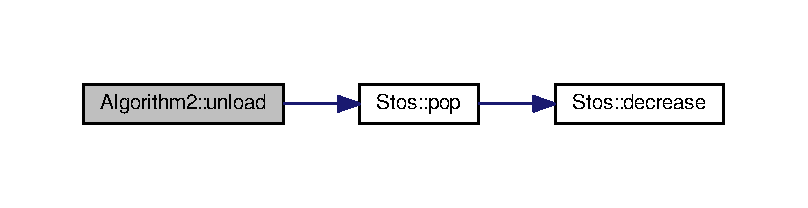
\includegraphics[width=350pt]{class_algorithm2_a3d7e4d0c9308d0b97250cb5596a73165_cgraph}
\end{center}
\end{figure}




\subsection{Dokumentacja atrybutów składowych}
\hypertarget{class_algorithm2_aff7c12a2dc0294d120a36ae0efc4af6a}{\index{Algorithm2@{Algorithm2}!tree@{tree}}
\index{tree@{tree}!Algorithm2@{Algorithm2}}
\subsubsection[{tree}]{\setlength{\rightskip}{0pt plus 5cm}{\bf Binary\-Tree} Algorithm2\-::tree\hspace{0.3cm}{\ttfamily [private]}}}\label{class_algorithm2_aff7c12a2dc0294d120a36ae0efc4af6a}


Definicja w linii 14 pliku algorithm2.\-hh.



Dokumentacja dla tej klasy została wygenerowana z plików\-:\begin{DoxyCompactItemize}
\item 
\hyperlink{algorithm2_8hh}{algorithm2.\-hh}\item 
\hyperlink{algorithm2_8cpp}{algorithm2.\-cpp}\end{DoxyCompactItemize}

\hypertarget{class_algorithm_kolejka}{\section{Dokumentacja klasy Algorithm\-Kolejka}
\label{class_algorithm_kolejka}\index{Algorithm\-Kolejka@{Algorithm\-Kolejka}}
}


Klasa \hyperlink{class_algorithm_kolejka}{Algorithm\-Kolejka} modelujaca algorytm wczytywania do kolejki. Obiekt tego typu reprezentuje algorytm wykonujacy wykonujacy wczytywanie zadanej ilosci elementow do kolejki.  




{\ttfamily \#include $<$algorithm\-\_\-kolejka.\-hh$>$}



Diagram dziedziczenia dla Algorithm\-Kolejka\nopagebreak
\begin{figure}[H]
\begin{center}
\leavevmode
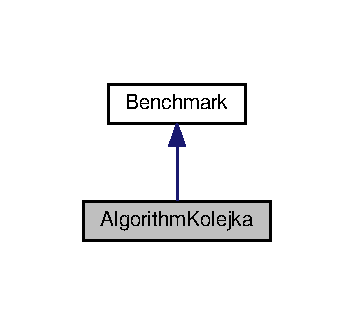
\includegraphics[width=170pt]{class_algorithm_kolejka__inherit__graph}
\end{center}
\end{figure}


Diagram współpracy dla Algorithm\-Kolejka\-:\nopagebreak
\begin{figure}[H]
\begin{center}
\leavevmode
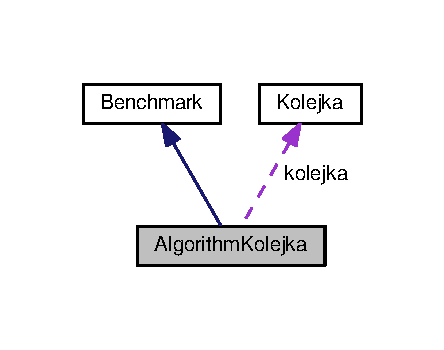
\includegraphics[width=213pt]{class_algorithm_kolejka__coll__graph}
\end{center}
\end{figure}
\subsection*{Metody publiczne}
\begin{DoxyCompactItemize}
\item 
\hyperlink{class_algorithm_kolejka_a024b4d14ce3e46ad167fa1961168088e}{Algorithm\-Kolejka} ()
\begin{DoxyCompactList}\small\item\em Konstruktor obiektu \hyperlink{class_algorithm_kolejka}{Algorithm\-Kolejka}. \end{DoxyCompactList}\item 
\hyperlink{class_algorithm_kolejka_a734671abcf48ef75dd1df980b503e618}{Algorithm\-Kolejka} (int \-\_\-tab\mbox{[}$\,$\mbox{]})
\begin{DoxyCompactList}\small\item\em Konstruktor parametryczny obiektu \hyperlink{class_algorithm_kolejka}{Algorithm\-Kolejka}. \end{DoxyCompactList}\item 
\hyperlink{class_algorithm_kolejka_a1df769a80bf632f57437c8d0cf6874d2}{$\sim$\-Algorithm\-Kolejka} ()
\begin{DoxyCompactList}\small\item\em Destruktor obiektu \hyperlink{class_algorithm_kolejka}{Algorithm\-Kolejka}. \end{DoxyCompactList}\item 
virtual void \hyperlink{class_algorithm_kolejka_ac739a8c865d4b71232549d12e0f1f466}{test\-Algorithm} (\hyperlink{class_benchmark}{Benchmark} $\ast$\-\_\-algorithm)
\begin{DoxyCompactList}\small\item\em Metoda testowania algorytmu. Metoda sluzy do testowania szybkosci dzialania algorytmu. W klasie \hyperlink{class_algorithm_kolejka}{Algorithm\-Kolejka} nie ma konkretnego dzialania. \end{DoxyCompactList}\item 
virtual void \hyperlink{class_algorithm_kolejka_ae9da3f1862fd90feb4a3c1d6b4f3dd8d}{run\-Algorithm} (int \-\_\-border)
\begin{DoxyCompactList}\small\item\em Metoda uruchamiania algorytmu. Metoda sluzy to wykonywania danego algorytmu. Wczytuje elementy do kolejki. \end{DoxyCompactList}\end{DoxyCompactItemize}
\subsection*{Atrybuty prywatne}
\begin{DoxyCompactItemize}
\item 
int \hyperlink{class_algorithm_kolejka_a12512e397f0f154464dc42fb060fdd3e}{tab} \mbox{[}\hyperlink{benchmark_8hh_a70ed59adcb4159ac551058053e649640}{S\-I\-Z\-E}\mbox{]}
\begin{DoxyCompactList}\small\item\em Tablica elementow z danymi wejsciowymi. \end{DoxyCompactList}\item 
\hyperlink{class_kolejka}{Kolejka} \hyperlink{class_algorithm_kolejka_a49a2b654776c15b98475ce3a7491c3ed}{kolejka}
\begin{DoxyCompactList}\small\item\em Zmienna przechowujaca kolejke. \end{DoxyCompactList}\end{DoxyCompactItemize}


\subsection{Opis szczegółowy}


Definicja w linii 9 pliku algorithm\-\_\-kolejka.\-hh.



\subsection{Dokumentacja konstruktora i destruktora}
\hypertarget{class_algorithm_kolejka_a024b4d14ce3e46ad167fa1961168088e}{\index{Algorithm\-Kolejka@{Algorithm\-Kolejka}!Algorithm\-Kolejka@{Algorithm\-Kolejka}}
\index{Algorithm\-Kolejka@{Algorithm\-Kolejka}!AlgorithmKolejka@{Algorithm\-Kolejka}}
\subsubsection[{Algorithm\-Kolejka}]{\setlength{\rightskip}{0pt plus 5cm}Algorithm\-Kolejka\-::\-Algorithm\-Kolejka (
\begin{DoxyParamCaption}
{}
\end{DoxyParamCaption}
)\hspace{0.3cm}{\ttfamily [inline]}}}\label{class_algorithm_kolejka_a024b4d14ce3e46ad167fa1961168088e}


Definicja w linii 24 pliku algorithm\-\_\-kolejka.\-hh.

\hypertarget{class_algorithm_kolejka_a734671abcf48ef75dd1df980b503e618}{\index{Algorithm\-Kolejka@{Algorithm\-Kolejka}!Algorithm\-Kolejka@{Algorithm\-Kolejka}}
\index{Algorithm\-Kolejka@{Algorithm\-Kolejka}!AlgorithmKolejka@{Algorithm\-Kolejka}}
\subsubsection[{Algorithm\-Kolejka}]{\setlength{\rightskip}{0pt plus 5cm}Algorithm\-Kolejka\-::\-Algorithm\-Kolejka (
\begin{DoxyParamCaption}
\item[{int}]{\-\_\-tab\mbox{[}$\,$\mbox{]}}
\end{DoxyParamCaption}
)\hspace{0.3cm}{\ttfamily [inline]}}}\label{class_algorithm_kolejka_a734671abcf48ef75dd1df980b503e618}

\begin{DoxyParams}[1]{Parametry}
\mbox{\tt in}  & {\em \-\_\-tab} & -\/ tablica przechowujaca dane wejsciowe. \\
\hline
\end{DoxyParams}


Definicja w linii 30 pliku algorithm\-\_\-kolejka.\-hh.

\hypertarget{class_algorithm_kolejka_a1df769a80bf632f57437c8d0cf6874d2}{\index{Algorithm\-Kolejka@{Algorithm\-Kolejka}!$\sim$\-Algorithm\-Kolejka@{$\sim$\-Algorithm\-Kolejka}}
\index{$\sim$\-Algorithm\-Kolejka@{$\sim$\-Algorithm\-Kolejka}!AlgorithmKolejka@{Algorithm\-Kolejka}}
\subsubsection[{$\sim$\-Algorithm\-Kolejka}]{\setlength{\rightskip}{0pt plus 5cm}Algorithm\-Kolejka\-::$\sim$\-Algorithm\-Kolejka (
\begin{DoxyParamCaption}
{}
\end{DoxyParamCaption}
)\hspace{0.3cm}{\ttfamily [inline]}}}\label{class_algorithm_kolejka_a1df769a80bf632f57437c8d0cf6874d2}


Definicja w linii 35 pliku algorithm\-\_\-kolejka.\-hh.



\subsection{Dokumentacja funkcji składowych}
\hypertarget{class_algorithm_kolejka_ae9da3f1862fd90feb4a3c1d6b4f3dd8d}{\index{Algorithm\-Kolejka@{Algorithm\-Kolejka}!run\-Algorithm@{run\-Algorithm}}
\index{run\-Algorithm@{run\-Algorithm}!AlgorithmKolejka@{Algorithm\-Kolejka}}
\subsubsection[{run\-Algorithm}]{\setlength{\rightskip}{0pt plus 5cm}void Algorithm\-Kolejka\-::run\-Algorithm (
\begin{DoxyParamCaption}
\item[{int}]{\-\_\-border}
\end{DoxyParamCaption}
)\hspace{0.3cm}{\ttfamily [virtual]}}}\label{class_algorithm_kolejka_ae9da3f1862fd90feb4a3c1d6b4f3dd8d}

\begin{DoxyParams}[1]{Parametry}
\mbox{\tt in}  & {\em \-\_\-border} & -\/ ilosc elementow dla ktorych algorytm ma wykonac swoje dzialanie. \\
\hline
\end{DoxyParams}


Reimplementowana z \hyperlink{class_benchmark_a6363894c058e8bfe146de09d7126b29c}{Benchmark}.



Definicja w linii 9 pliku algorithm\-\_\-kolejka.\-cpp.



Oto graf wywołań dla tej funkcji\-:\nopagebreak
\begin{figure}[H]
\begin{center}
\leavevmode
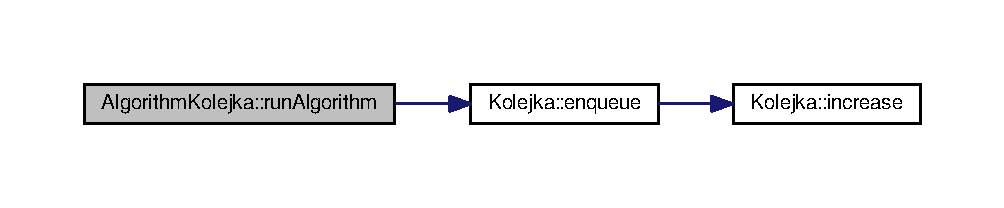
\includegraphics[width=350pt]{class_algorithm_kolejka_ae9da3f1862fd90feb4a3c1d6b4f3dd8d_cgraph}
\end{center}
\end{figure}


\hypertarget{class_algorithm_kolejka_ac739a8c865d4b71232549d12e0f1f466}{\index{Algorithm\-Kolejka@{Algorithm\-Kolejka}!test\-Algorithm@{test\-Algorithm}}
\index{test\-Algorithm@{test\-Algorithm}!AlgorithmKolejka@{Algorithm\-Kolejka}}
\subsubsection[{test\-Algorithm}]{\setlength{\rightskip}{0pt plus 5cm}virtual void Algorithm\-Kolejka\-::test\-Algorithm (
\begin{DoxyParamCaption}
\item[{{\bf Benchmark} $\ast$}]{\-\_\-algorithm}
\end{DoxyParamCaption}
)\hspace{0.3cm}{\ttfamily [inline]}, {\ttfamily [virtual]}}}\label{class_algorithm_kolejka_ac739a8c865d4b71232549d12e0f1f466}

\begin{DoxyParams}[1]{Parametry}
\mbox{\tt in}  & {\em \-\_\-algorithm} & -\/ testowany algorytm. \\
\hline
\end{DoxyParams}


Definicja w linii 43 pliku algorithm\-\_\-kolejka.\-hh.



\subsection{Dokumentacja atrybutów składowych}
\hypertarget{class_algorithm_kolejka_a49a2b654776c15b98475ce3a7491c3ed}{\index{Algorithm\-Kolejka@{Algorithm\-Kolejka}!kolejka@{kolejka}}
\index{kolejka@{kolejka}!AlgorithmKolejka@{Algorithm\-Kolejka}}
\subsubsection[{kolejka}]{\setlength{\rightskip}{0pt plus 5cm}{\bf Kolejka} Algorithm\-Kolejka\-::kolejka\hspace{0.3cm}{\ttfamily [private]}}}\label{class_algorithm_kolejka_a49a2b654776c15b98475ce3a7491c3ed}


Definicja w linii 18 pliku algorithm\-\_\-kolejka.\-hh.

\hypertarget{class_algorithm_kolejka_a12512e397f0f154464dc42fb060fdd3e}{\index{Algorithm\-Kolejka@{Algorithm\-Kolejka}!tab@{tab}}
\index{tab@{tab}!AlgorithmKolejka@{Algorithm\-Kolejka}}
\subsubsection[{tab}]{\setlength{\rightskip}{0pt plus 5cm}int Algorithm\-Kolejka\-::tab\mbox{[}{\bf S\-I\-Z\-E}\mbox{]}\hspace{0.3cm}{\ttfamily [private]}}}\label{class_algorithm_kolejka_a12512e397f0f154464dc42fb060fdd3e}


Definicja w linii 14 pliku algorithm\-\_\-kolejka.\-hh.



Dokumentacja dla tej klasy została wygenerowana z plików\-:\begin{DoxyCompactItemize}
\item 
\hyperlink{algorithm__kolejka_8hh}{algorithm\-\_\-kolejka.\-hh}\item 
\hyperlink{algorithm__kolejka_8cpp}{algorithm\-\_\-kolejka.\-cpp}\end{DoxyCompactItemize}

\hypertarget{class_algorithm_lista}{\section{Dokumentacja klasy Algorithm\-Lista}
\label{class_algorithm_lista}\index{Algorithm\-Lista@{Algorithm\-Lista}}
}


Klasa \hyperlink{class_algorithm_lista}{Algorithm\-Lista} modelujaca algorytm wczytywania do kolejki. Obiekt tego typu reprezentuje algorytm wykonujacy wykonujacy wczytywanie zadanej ilosci elementow do listy.  




{\ttfamily \#include $<$algorithm\-\_\-lista.\-hh$>$}



Diagram dziedziczenia dla Algorithm\-Lista\nopagebreak
\begin{figure}[H]
\begin{center}
\leavevmode
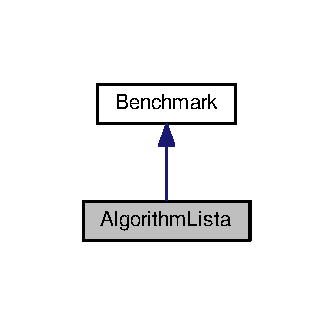
\includegraphics[width=160pt]{class_algorithm_lista__inherit__graph}
\end{center}
\end{figure}


Diagram współpracy dla Algorithm\-Lista\-:\nopagebreak
\begin{figure}[H]
\begin{center}
\leavevmode
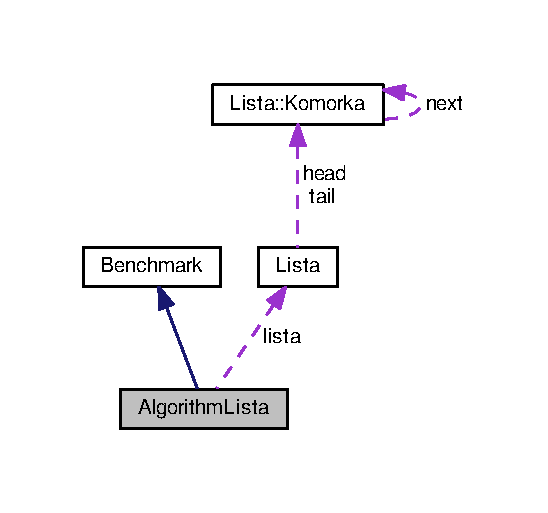
\includegraphics[width=263pt]{class_algorithm_lista__coll__graph}
\end{center}
\end{figure}
\subsection*{Metody publiczne}
\begin{DoxyCompactItemize}
\item 
\hyperlink{class_algorithm_lista_a4c7749379de38154982288419f305141}{Algorithm\-Lista} ()
\begin{DoxyCompactList}\small\item\em Konstruktor obiektu \hyperlink{class_algorithm_lista}{Algorithm\-Lista}. \end{DoxyCompactList}\item 
\hyperlink{class_algorithm_lista_ab5aed5527ca4f27c213e97fa19f6e32d}{Algorithm\-Lista} (int \-\_\-tab\mbox{[}$\,$\mbox{]})
\begin{DoxyCompactList}\small\item\em Konstruktor parametryczny obiektu \hyperlink{class_algorithm_lista}{Algorithm\-Lista}. \end{DoxyCompactList}\item 
\hyperlink{class_algorithm_lista_a2d7c5ef95cdfe523a86b01da06d0fb2e}{$\sim$\-Algorithm\-Lista} ()
\begin{DoxyCompactList}\small\item\em Destruktor obiektu \hyperlink{class_algorithm_lista}{Algorithm\-Lista}. \end{DoxyCompactList}\item 
virtual void \hyperlink{class_algorithm_lista_a1e1f93e75b4a635098bf30ec32f19903}{test\-Algorithm} (\hyperlink{class_benchmark}{Benchmark} $\ast$\-\_\-algorithm)
\begin{DoxyCompactList}\small\item\em Metoda testowania algorytmu. Metoda sluzy do testowania szybkosci dzialania algorytmu. W klasie \hyperlink{class_algorithm_lista}{Algorithm\-Lista} nie ma konkretnego dzialania. \end{DoxyCompactList}\item 
virtual void \hyperlink{class_algorithm_lista_a5c41dbbd3ae7a9ac34edec1a51bc8eb1}{run\-Algorithm} (int \-\_\-border)
\begin{DoxyCompactList}\small\item\em Metoda uruchamiania algorytmu. Metoda sluzy to wykonywania danego algorytmu. Wczytuje elementy do kolejki. \end{DoxyCompactList}\end{DoxyCompactItemize}
\subsection*{Atrybuty prywatne}
\begin{DoxyCompactItemize}
\item 
int \hyperlink{class_algorithm_lista_ad04d74953d75c8886b0c5cfda71773f7}{tab} \mbox{[}\hyperlink{benchmark_8hh_a70ed59adcb4159ac551058053e649640}{S\-I\-Z\-E}\mbox{]}
\begin{DoxyCompactList}\small\item\em Tablica elementow z danymi wejsciowymi. \end{DoxyCompactList}\item 
\hyperlink{class_lista}{Lista} \hyperlink{class_algorithm_lista_a5c4c8b55e6d71eae06c98cd39f38bb30}{lista}
\begin{DoxyCompactList}\small\item\em Zmienna przechowujaca liste. \end{DoxyCompactList}\end{DoxyCompactItemize}


\subsection{Opis szczegółowy}


Definicja w linii 9 pliku algorithm\-\_\-lista.\-hh.



\subsection{Dokumentacja konstruktora i destruktora}
\hypertarget{class_algorithm_lista_a4c7749379de38154982288419f305141}{\index{Algorithm\-Lista@{Algorithm\-Lista}!Algorithm\-Lista@{Algorithm\-Lista}}
\index{Algorithm\-Lista@{Algorithm\-Lista}!AlgorithmLista@{Algorithm\-Lista}}
\subsubsection[{Algorithm\-Lista}]{\setlength{\rightskip}{0pt plus 5cm}Algorithm\-Lista\-::\-Algorithm\-Lista (
\begin{DoxyParamCaption}
{}
\end{DoxyParamCaption}
)\hspace{0.3cm}{\ttfamily [inline]}}}\label{class_algorithm_lista_a4c7749379de38154982288419f305141}


Definicja w linii 24 pliku algorithm\-\_\-lista.\-hh.

\hypertarget{class_algorithm_lista_ab5aed5527ca4f27c213e97fa19f6e32d}{\index{Algorithm\-Lista@{Algorithm\-Lista}!Algorithm\-Lista@{Algorithm\-Lista}}
\index{Algorithm\-Lista@{Algorithm\-Lista}!AlgorithmLista@{Algorithm\-Lista}}
\subsubsection[{Algorithm\-Lista}]{\setlength{\rightskip}{0pt plus 5cm}Algorithm\-Lista\-::\-Algorithm\-Lista (
\begin{DoxyParamCaption}
\item[{int}]{\-\_\-tab\mbox{[}$\,$\mbox{]}}
\end{DoxyParamCaption}
)\hspace{0.3cm}{\ttfamily [inline]}}}\label{class_algorithm_lista_ab5aed5527ca4f27c213e97fa19f6e32d}

\begin{DoxyParams}[1]{Parametry}
\mbox{\tt in}  & {\em \-\_\-tab} & -\/ tablica przechowujaca dane wejsciowe. \\
\hline
\end{DoxyParams}


Definicja w linii 30 pliku algorithm\-\_\-lista.\-hh.

\hypertarget{class_algorithm_lista_a2d7c5ef95cdfe523a86b01da06d0fb2e}{\index{Algorithm\-Lista@{Algorithm\-Lista}!$\sim$\-Algorithm\-Lista@{$\sim$\-Algorithm\-Lista}}
\index{$\sim$\-Algorithm\-Lista@{$\sim$\-Algorithm\-Lista}!AlgorithmLista@{Algorithm\-Lista}}
\subsubsection[{$\sim$\-Algorithm\-Lista}]{\setlength{\rightskip}{0pt plus 5cm}Algorithm\-Lista\-::$\sim$\-Algorithm\-Lista (
\begin{DoxyParamCaption}
{}
\end{DoxyParamCaption}
)\hspace{0.3cm}{\ttfamily [inline]}}}\label{class_algorithm_lista_a2d7c5ef95cdfe523a86b01da06d0fb2e}


Definicja w linii 35 pliku algorithm\-\_\-lista.\-hh.



\subsection{Dokumentacja funkcji składowych}
\hypertarget{class_algorithm_lista_a5c41dbbd3ae7a9ac34edec1a51bc8eb1}{\index{Algorithm\-Lista@{Algorithm\-Lista}!run\-Algorithm@{run\-Algorithm}}
\index{run\-Algorithm@{run\-Algorithm}!AlgorithmLista@{Algorithm\-Lista}}
\subsubsection[{run\-Algorithm}]{\setlength{\rightskip}{0pt plus 5cm}void Algorithm\-Lista\-::run\-Algorithm (
\begin{DoxyParamCaption}
\item[{int}]{\-\_\-border}
\end{DoxyParamCaption}
)\hspace{0.3cm}{\ttfamily [virtual]}}}\label{class_algorithm_lista_a5c41dbbd3ae7a9ac34edec1a51bc8eb1}

\begin{DoxyParams}[1]{Parametry}
\mbox{\tt in}  & {\em \-\_\-border} & -\/ ilosc elementow dla ktorych algorytm ma wykonac swoje dzialanie. \\
\hline
\end{DoxyParams}


Reimplementowana z \hyperlink{class_benchmark_a6363894c058e8bfe146de09d7126b29c}{Benchmark}.



Definicja w linii 8 pliku algorithm\-\_\-lista.\-cpp.



Oto graf wywołań dla tej funkcji\-:\nopagebreak
\begin{figure}[H]
\begin{center}
\leavevmode
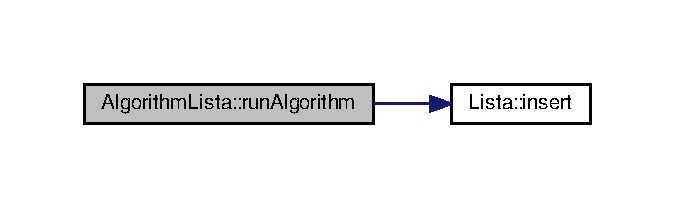
\includegraphics[width=324pt]{class_algorithm_lista_a5c41dbbd3ae7a9ac34edec1a51bc8eb1_cgraph}
\end{center}
\end{figure}


\hypertarget{class_algorithm_lista_a1e1f93e75b4a635098bf30ec32f19903}{\index{Algorithm\-Lista@{Algorithm\-Lista}!test\-Algorithm@{test\-Algorithm}}
\index{test\-Algorithm@{test\-Algorithm}!AlgorithmLista@{Algorithm\-Lista}}
\subsubsection[{test\-Algorithm}]{\setlength{\rightskip}{0pt plus 5cm}virtual void Algorithm\-Lista\-::test\-Algorithm (
\begin{DoxyParamCaption}
\item[{{\bf Benchmark} $\ast$}]{\-\_\-algorithm}
\end{DoxyParamCaption}
)\hspace{0.3cm}{\ttfamily [inline]}, {\ttfamily [virtual]}}}\label{class_algorithm_lista_a1e1f93e75b4a635098bf30ec32f19903}

\begin{DoxyParams}[1]{Parametry}
\mbox{\tt in}  & {\em \-\_\-algorithm} & -\/ testowany algorytm. \\
\hline
\end{DoxyParams}


Definicja w linii 43 pliku algorithm\-\_\-lista.\-hh.



\subsection{Dokumentacja atrybutów składowych}
\hypertarget{class_algorithm_lista_a5c4c8b55e6d71eae06c98cd39f38bb30}{\index{Algorithm\-Lista@{Algorithm\-Lista}!lista@{lista}}
\index{lista@{lista}!AlgorithmLista@{Algorithm\-Lista}}
\subsubsection[{lista}]{\setlength{\rightskip}{0pt plus 5cm}{\bf Lista} Algorithm\-Lista\-::lista\hspace{0.3cm}{\ttfamily [private]}}}\label{class_algorithm_lista_a5c4c8b55e6d71eae06c98cd39f38bb30}


Definicja w linii 18 pliku algorithm\-\_\-lista.\-hh.

\hypertarget{class_algorithm_lista_ad04d74953d75c8886b0c5cfda71773f7}{\index{Algorithm\-Lista@{Algorithm\-Lista}!tab@{tab}}
\index{tab@{tab}!AlgorithmLista@{Algorithm\-Lista}}
\subsubsection[{tab}]{\setlength{\rightskip}{0pt plus 5cm}int Algorithm\-Lista\-::tab\mbox{[}{\bf S\-I\-Z\-E}\mbox{]}\hspace{0.3cm}{\ttfamily [private]}}}\label{class_algorithm_lista_ad04d74953d75c8886b0c5cfda71773f7}


Definicja w linii 14 pliku algorithm\-\_\-lista.\-hh.



Dokumentacja dla tej klasy została wygenerowana z plików\-:\begin{DoxyCompactItemize}
\item 
\hyperlink{algorithm__lista_8hh}{algorithm\-\_\-lista.\-hh}\item 
\hyperlink{algorithm__lista_8cpp}{algorithm\-\_\-lista.\-cpp}\end{DoxyCompactItemize}

\hypertarget{class_algorithm_stos}{\section{Dokumentacja klasy Algorithm\-Stos}
\label{class_algorithm_stos}\index{Algorithm\-Stos@{Algorithm\-Stos}}
}


Klasa \hyperlink{class_algorithm_stos}{Algorithm\-Stos} modelujaca algorytm wczytywania do stosu. Obiekt tego typu reprezentuje algorytm wykonujacy wykonujacy wczytywanie zadanej ilosci elementow do stosu.  




{\ttfamily \#include $<$algorithm\-\_\-stos.\-hh$>$}



Diagram dziedziczenia dla Algorithm\-Stos\nopagebreak
\begin{figure}[H]
\begin{center}
\leavevmode
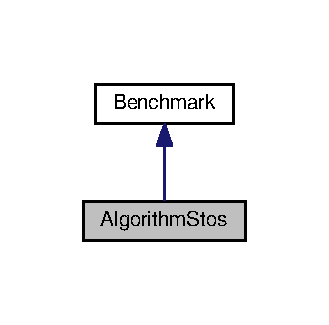
\includegraphics[width=158pt]{class_algorithm_stos__inherit__graph}
\end{center}
\end{figure}


Diagram współpracy dla Algorithm\-Stos\-:\nopagebreak
\begin{figure}[H]
\begin{center}
\leavevmode
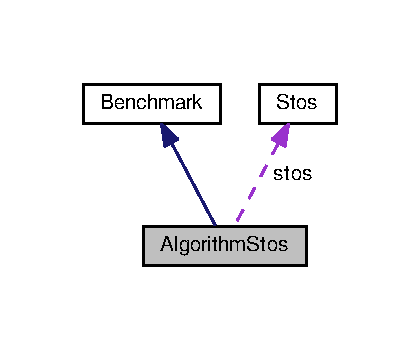
\includegraphics[width=201pt]{class_algorithm_stos__coll__graph}
\end{center}
\end{figure}
\subsection*{Metody publiczne}
\begin{DoxyCompactItemize}
\item 
\hyperlink{class_algorithm_stos_a0d987377d7c5d9cea3152680ba437cd3}{Algorithm\-Stos} ()
\begin{DoxyCompactList}\small\item\em Konstruktor obiektu \hyperlink{class_algorithm_stos}{Algorithm\-Stos}. \end{DoxyCompactList}\item 
\hyperlink{class_algorithm_stos_a5dc7ad87d403c67d64aa6cac6a626992}{Algorithm\-Stos} (int \-\_\-tab\mbox{[}$\,$\mbox{]})
\begin{DoxyCompactList}\small\item\em Konstruktor parametryczny obiektu \hyperlink{class_algorithm_stos}{Algorithm\-Stos}. \end{DoxyCompactList}\item 
\hyperlink{class_algorithm_stos_a68a3733d5dfd9fefe38059f0ce0202bf}{$\sim$\-Algorithm\-Stos} ()
\begin{DoxyCompactList}\small\item\em Destruktor obiektu \hyperlink{class_algorithm_stos}{Algorithm\-Stos}. \end{DoxyCompactList}\item 
virtual void \hyperlink{class_algorithm_stos_a7fb987baf970d51f90ad880d27e537a4}{test\-Algorithm} (\hyperlink{class_benchmark}{Benchmark} $\ast$\-\_\-algorithm)
\begin{DoxyCompactList}\small\item\em Metoda testowania algorytmu. Metoda sluzy do testowania szybkosci dzialania algorytmu. W klasie \hyperlink{class_algorithm_stos}{Algorithm\-Stos} nie ma konkretnego dzialania. \end{DoxyCompactList}\item 
virtual void \hyperlink{class_algorithm_stos_a889f7150ae3651b40e5acca7542dbbd1}{run\-Algorithm} (int \-\_\-border)
\begin{DoxyCompactList}\small\item\em Metoda uruchamiania algorytmu. Metoda sluzy to wykonywania danego algorytmu. Wczytuje elementy do stosu. \end{DoxyCompactList}\end{DoxyCompactItemize}
\subsection*{Atrybuty prywatne}
\begin{DoxyCompactItemize}
\item 
int \hyperlink{class_algorithm_stos_a2fb5db929aa54bf64794c812830d8648}{tab} \mbox{[}\hyperlink{benchmark_8hh_a70ed59adcb4159ac551058053e649640}{S\-I\-Z\-E}\mbox{]}
\begin{DoxyCompactList}\small\item\em Tablica elementow z danymi wejsciowymi. \end{DoxyCompactList}\item 
\hyperlink{class_stos}{Stos} \hyperlink{class_algorithm_stos_a0b803ecc25fd3586cf07969697367754}{stos}
\begin{DoxyCompactList}\small\item\em Zmienna przechowujaca stos. \end{DoxyCompactList}\end{DoxyCompactItemize}


\subsection{Opis szczegółowy}


Definicja w linii 9 pliku algorithm\-\_\-stos.\-hh.



\subsection{Dokumentacja konstruktora i destruktora}
\hypertarget{class_algorithm_stos_a0d987377d7c5d9cea3152680ba437cd3}{\index{Algorithm\-Stos@{Algorithm\-Stos}!Algorithm\-Stos@{Algorithm\-Stos}}
\index{Algorithm\-Stos@{Algorithm\-Stos}!AlgorithmStos@{Algorithm\-Stos}}
\subsubsection[{Algorithm\-Stos}]{\setlength{\rightskip}{0pt plus 5cm}Algorithm\-Stos\-::\-Algorithm\-Stos (
\begin{DoxyParamCaption}
{}
\end{DoxyParamCaption}
)\hspace{0.3cm}{\ttfamily [inline]}}}\label{class_algorithm_stos_a0d987377d7c5d9cea3152680ba437cd3}


Definicja w linii 24 pliku algorithm\-\_\-stos.\-hh.

\hypertarget{class_algorithm_stos_a5dc7ad87d403c67d64aa6cac6a626992}{\index{Algorithm\-Stos@{Algorithm\-Stos}!Algorithm\-Stos@{Algorithm\-Stos}}
\index{Algorithm\-Stos@{Algorithm\-Stos}!AlgorithmStos@{Algorithm\-Stos}}
\subsubsection[{Algorithm\-Stos}]{\setlength{\rightskip}{0pt plus 5cm}Algorithm\-Stos\-::\-Algorithm\-Stos (
\begin{DoxyParamCaption}
\item[{int}]{\-\_\-tab\mbox{[}$\,$\mbox{]}}
\end{DoxyParamCaption}
)\hspace{0.3cm}{\ttfamily [inline]}}}\label{class_algorithm_stos_a5dc7ad87d403c67d64aa6cac6a626992}

\begin{DoxyParams}[1]{Parametry}
\mbox{\tt in}  & {\em \-\_\-tab} & -\/ tablica przechowujaca dane wejsciowe. \\
\hline
\end{DoxyParams}


Definicja w linii 30 pliku algorithm\-\_\-stos.\-hh.

\hypertarget{class_algorithm_stos_a68a3733d5dfd9fefe38059f0ce0202bf}{\index{Algorithm\-Stos@{Algorithm\-Stos}!$\sim$\-Algorithm\-Stos@{$\sim$\-Algorithm\-Stos}}
\index{$\sim$\-Algorithm\-Stos@{$\sim$\-Algorithm\-Stos}!AlgorithmStos@{Algorithm\-Stos}}
\subsubsection[{$\sim$\-Algorithm\-Stos}]{\setlength{\rightskip}{0pt plus 5cm}Algorithm\-Stos\-::$\sim$\-Algorithm\-Stos (
\begin{DoxyParamCaption}
{}
\end{DoxyParamCaption}
)\hspace{0.3cm}{\ttfamily [inline]}}}\label{class_algorithm_stos_a68a3733d5dfd9fefe38059f0ce0202bf}


Definicja w linii 35 pliku algorithm\-\_\-stos.\-hh.



\subsection{Dokumentacja funkcji składowych}
\hypertarget{class_algorithm_stos_a889f7150ae3651b40e5acca7542dbbd1}{\index{Algorithm\-Stos@{Algorithm\-Stos}!run\-Algorithm@{run\-Algorithm}}
\index{run\-Algorithm@{run\-Algorithm}!AlgorithmStos@{Algorithm\-Stos}}
\subsubsection[{run\-Algorithm}]{\setlength{\rightskip}{0pt plus 5cm}void Algorithm\-Stos\-::run\-Algorithm (
\begin{DoxyParamCaption}
\item[{int}]{\-\_\-border}
\end{DoxyParamCaption}
)\hspace{0.3cm}{\ttfamily [virtual]}}}\label{class_algorithm_stos_a889f7150ae3651b40e5acca7542dbbd1}

\begin{DoxyParams}[1]{Parametry}
\mbox{\tt in}  & {\em \-\_\-border} & -\/ ilosc elementow dla ktorych algorytm ma wykonac swoje dzialanie. \\
\hline
\end{DoxyParams}


Reimplementowana z \hyperlink{class_benchmark_a6363894c058e8bfe146de09d7126b29c}{Benchmark}.



Definicja w linii 9 pliku algorithm\-\_\-stos.\-cpp.



Oto graf wywołań dla tej funkcji\-:\nopagebreak
\begin{figure}[H]
\begin{center}
\leavevmode
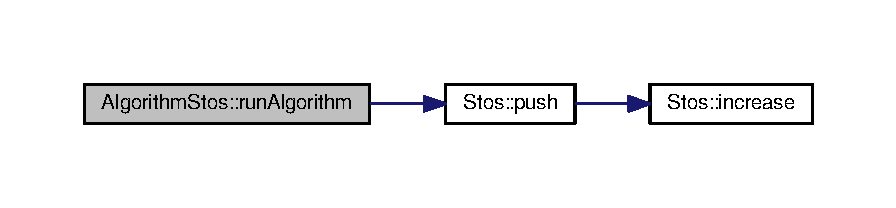
\includegraphics[width=350pt]{class_algorithm_stos_a889f7150ae3651b40e5acca7542dbbd1_cgraph}
\end{center}
\end{figure}


\hypertarget{class_algorithm_stos_a7fb987baf970d51f90ad880d27e537a4}{\index{Algorithm\-Stos@{Algorithm\-Stos}!test\-Algorithm@{test\-Algorithm}}
\index{test\-Algorithm@{test\-Algorithm}!AlgorithmStos@{Algorithm\-Stos}}
\subsubsection[{test\-Algorithm}]{\setlength{\rightskip}{0pt plus 5cm}virtual void Algorithm\-Stos\-::test\-Algorithm (
\begin{DoxyParamCaption}
\item[{{\bf Benchmark} $\ast$}]{\-\_\-algorithm}
\end{DoxyParamCaption}
)\hspace{0.3cm}{\ttfamily [inline]}, {\ttfamily [virtual]}}}\label{class_algorithm_stos_a7fb987baf970d51f90ad880d27e537a4}

\begin{DoxyParams}[1]{Parametry}
\mbox{\tt in}  & {\em \-\_\-algorithm} & -\/ testowany algorytm. \\
\hline
\end{DoxyParams}


Definicja w linii 43 pliku algorithm\-\_\-stos.\-hh.



\subsection{Dokumentacja atrybutów składowych}
\hypertarget{class_algorithm_stos_a0b803ecc25fd3586cf07969697367754}{\index{Algorithm\-Stos@{Algorithm\-Stos}!stos@{stos}}
\index{stos@{stos}!AlgorithmStos@{Algorithm\-Stos}}
\subsubsection[{stos}]{\setlength{\rightskip}{0pt plus 5cm}{\bf Stos} Algorithm\-Stos\-::stos\hspace{0.3cm}{\ttfamily [private]}}}\label{class_algorithm_stos_a0b803ecc25fd3586cf07969697367754}


Definicja w linii 18 pliku algorithm\-\_\-stos.\-hh.

\hypertarget{class_algorithm_stos_a2fb5db929aa54bf64794c812830d8648}{\index{Algorithm\-Stos@{Algorithm\-Stos}!tab@{tab}}
\index{tab@{tab}!AlgorithmStos@{Algorithm\-Stos}}
\subsubsection[{tab}]{\setlength{\rightskip}{0pt plus 5cm}int Algorithm\-Stos\-::tab\mbox{[}{\bf S\-I\-Z\-E}\mbox{]}\hspace{0.3cm}{\ttfamily [private]}}}\label{class_algorithm_stos_a2fb5db929aa54bf64794c812830d8648}


Definicja w linii 14 pliku algorithm\-\_\-stos.\-hh.



Dokumentacja dla tej klasy została wygenerowana z plików\-:\begin{DoxyCompactItemize}
\item 
\hyperlink{algorithm__stos_8hh}{algorithm\-\_\-stos.\-hh}\item 
\hyperlink{algorithm__stos_8cpp}{algorithm\-\_\-stos.\-cpp}\end{DoxyCompactItemize}

\hypertarget{class_benchmark}{\section{Dokumentacja klasy Benchmark}
\label{class_benchmark}\index{Benchmark@{Benchmark}}
}


Klasa \hyperlink{class_benchmark}{Benchmark} modelujaca program benchmarkujacy. Obiekt tego typu reprezentuje program sprawdzajacy szybkosc wykonywania algorytmow.  




{\ttfamily \#include $<$benchmark.\-hh$>$}



Diagram dziedziczenia dla Benchmark\nopagebreak
\begin{figure}[H]
\begin{center}
\leavevmode
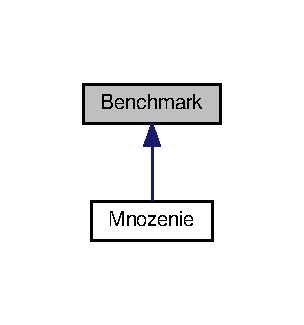
\includegraphics[width=350pt]{class_benchmark__inherit__graph}
\end{center}
\end{figure}
\subsection*{Metody publiczne}
\begin{DoxyCompactItemize}
\item 
\hyperlink{class_benchmark_acfca497989836a688d44477802e822d8}{Benchmark} ()
\begin{DoxyCompactList}\small\item\em Konstrukor obiektu \hyperlink{class_benchmark}{Benchmark}. \end{DoxyCompactList}\item 
\hyperlink{class_benchmark_a20476e07f09e2b20ed3e9a7f13a570e6}{$\sim$\-Benchmark} ()
\begin{DoxyCompactList}\small\item\em Destruktor obiektu \hyperlink{class_benchmark}{Benchmark}. \end{DoxyCompactList}\item 
virtual void \hyperlink{class_benchmark_a900bc0d26c2ed6aa45afe4d5b295ccd1}{test\-Algorithm} (\hyperlink{class_benchmark}{Benchmark} $\ast$\-\_\-algorithm, int \-\_\-n) const 
\begin{DoxyCompactList}\small\item\em Metoda testowania algorytmu. Metoda sluzy to testowania szybkosci dzialania algorytmu. Wykonuje testowany algorytm dla 5 kolejnych ilosci elementow. Wykonanie algorytmu dla danego zestawu liczb powtarza dwa razy i usrednia wynik. Otrzymany czas wraz z iloscia testowanych danych zapisuje w pliku ret\-\_\-data.\-txt. \end{DoxyCompactList}\item 
virtual void \hyperlink{class_benchmark_a6363894c058e8bfe146de09d7126b29c}{run\-Algorithm} (int \-\_\-border)
\begin{DoxyCompactList}\small\item\em Metoda uruchamiania algorytmu. Metoda sluzy do wykonywania danego algorytmu. W klasie \hyperlink{class_benchmark}{Benchmark} nie ma konkretnego dzialania. \end{DoxyCompactList}\end{DoxyCompactItemize}
\subsection*{Atrybuty prywatne}
\begin{DoxyCompactItemize}
\item 
std\-::string \hyperlink{class_benchmark_aee0beda65009e7334d34c5957f78c49a}{nazwy} \mbox{[}4\mbox{]} = \{\char`\"{}ret\-\_\-data1.\-txt\char`\"{}, \char`\"{}ret\-\_\-data2.\-txt\char`\"{}, \char`\"{}ret\-\_\-data3.\-txt\char`\"{}, \char`\"{}ret\-\_\-data4.\-txt\char`\"{}\}
\begin{DoxyCompactList}\small\item\em Tablica stringow przechowujaca nazwy plikow do zapisu. \end{DoxyCompactList}\end{DoxyCompactItemize}


\subsection{Opis szczegółowy}


Definicja w linii 11 pliku benchmark.\-hh.



\subsection{Dokumentacja konstruktora i destruktora}
\hypertarget{class_benchmark_acfca497989836a688d44477802e822d8}{\index{Benchmark@{Benchmark}!Benchmark@{Benchmark}}
\index{Benchmark@{Benchmark}!Benchmark@{Benchmark}}
\subsubsection[{Benchmark}]{\setlength{\rightskip}{0pt plus 5cm}Benchmark\-::\-Benchmark (
\begin{DoxyParamCaption}
{}
\end{DoxyParamCaption}
)\hspace{0.3cm}{\ttfamily [inline]}}}\label{class_benchmark_acfca497989836a688d44477802e822d8}


Definicja w linii 23 pliku benchmark.\-hh.

\hypertarget{class_benchmark_a20476e07f09e2b20ed3e9a7f13a570e6}{\index{Benchmark@{Benchmark}!$\sim$\-Benchmark@{$\sim$\-Benchmark}}
\index{$\sim$\-Benchmark@{$\sim$\-Benchmark}!Benchmark@{Benchmark}}
\subsubsection[{$\sim$\-Benchmark}]{\setlength{\rightskip}{0pt plus 5cm}Benchmark\-::$\sim$\-Benchmark (
\begin{DoxyParamCaption}
{}
\end{DoxyParamCaption}
)\hspace{0.3cm}{\ttfamily [inline]}}}\label{class_benchmark_a20476e07f09e2b20ed3e9a7f13a570e6}


Definicja w linii 28 pliku benchmark.\-hh.



\subsection{Dokumentacja funkcji składowych}
\hypertarget{class_benchmark_a6363894c058e8bfe146de09d7126b29c}{\index{Benchmark@{Benchmark}!run\-Algorithm@{run\-Algorithm}}
\index{run\-Algorithm@{run\-Algorithm}!Benchmark@{Benchmark}}
\subsubsection[{run\-Algorithm}]{\setlength{\rightskip}{0pt plus 5cm}virtual void Benchmark\-::run\-Algorithm (
\begin{DoxyParamCaption}
\item[{int}]{\-\_\-border}
\end{DoxyParamCaption}
)\hspace{0.3cm}{\ttfamily [inline]}, {\ttfamily [virtual]}}}\label{class_benchmark_a6363894c058e8bfe146de09d7126b29c}

\begin{DoxyParams}[1]{Parametry}
\mbox{\tt in}  & {\em \-\_\-border} & -\/ ilosc elementow dla ktorych algorytm ma wykonac swoje dzialanie. \\
\hline
\end{DoxyParams}


Reimplementowana w \hyperlink{class_algorithm2_a409e58d5fb0b6d2407cc986cf163703b}{Algorithm2}, \hyperlink{class_algorithm_kolejka_ae9da3f1862fd90feb4a3c1d6b4f3dd8d}{Algorithm\-Kolejka}, \hyperlink{class_algorithm_lista_a5c41dbbd3ae7a9ac34edec1a51bc8eb1}{Algorithm\-Lista} i \hyperlink{class_algorithm_stos_a889f7150ae3651b40e5acca7542dbbd1}{Algorithm\-Stos}.



Definicja w linii 48 pliku benchmark.\-hh.



Oto graf wywoływań tej funkcji\-:\nopagebreak
\begin{figure}[H]
\begin{center}
\leavevmode
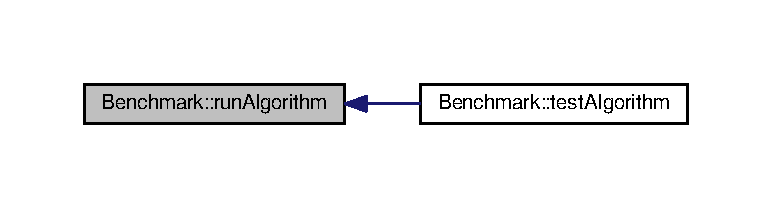
\includegraphics[width=350pt]{class_benchmark_a6363894c058e8bfe146de09d7126b29c_icgraph}
\end{center}
\end{figure}


\hypertarget{class_benchmark_a900bc0d26c2ed6aa45afe4d5b295ccd1}{\index{Benchmark@{Benchmark}!test\-Algorithm@{test\-Algorithm}}
\index{test\-Algorithm@{test\-Algorithm}!Benchmark@{Benchmark}}
\subsubsection[{test\-Algorithm}]{\setlength{\rightskip}{0pt plus 5cm}void Benchmark\-::test\-Algorithm (
\begin{DoxyParamCaption}
\item[{{\bf Benchmark} $\ast$}]{\-\_\-algorithm, }
\item[{int}]{\-\_\-n}
\end{DoxyParamCaption}
) const\hspace{0.3cm}{\ttfamily [virtual]}}}\label{class_benchmark_a900bc0d26c2ed6aa45afe4d5b295ccd1}

\begin{DoxyParams}[1]{Parametry}
\mbox{\tt in}  & {\em \-\_\-algorithm} & -\/ testowany algorytm. \\
\hline
\mbox{\tt in}  & {\em \-\_\-n} & -\/ indeks nazwy pliku \\
\hline
\end{DoxyParams}


Definicja w linii 12 pliku benchmark.\-cpp.



Oto graf wywołań dla tej funkcji\-:\nopagebreak
\begin{figure}[H]
\begin{center}
\leavevmode
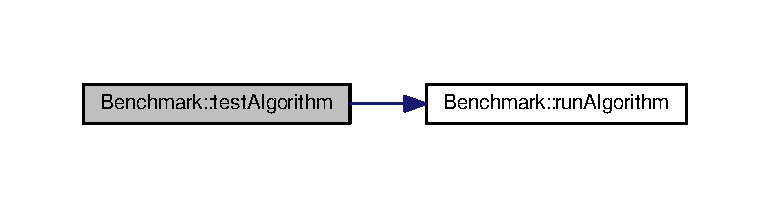
\includegraphics[width=350pt]{class_benchmark_a900bc0d26c2ed6aa45afe4d5b295ccd1_cgraph}
\end{center}
\end{figure}




\subsection{Dokumentacja atrybutów składowych}
\hypertarget{class_benchmark_aee0beda65009e7334d34c5957f78c49a}{\index{Benchmark@{Benchmark}!nazwy@{nazwy}}
\index{nazwy@{nazwy}!Benchmark@{Benchmark}}
\subsubsection[{nazwy}]{\setlength{\rightskip}{0pt plus 5cm}std\-::string Benchmark\-::nazwy\mbox{[}4\mbox{]} = \{\char`\"{}ret\-\_\-data1.\-txt\char`\"{}, \char`\"{}ret\-\_\-data2.\-txt\char`\"{}, \char`\"{}ret\-\_\-data3.\-txt\char`\"{}, \char`\"{}ret\-\_\-data4.\-txt\char`\"{}\}\hspace{0.3cm}{\ttfamily [private]}}}\label{class_benchmark_aee0beda65009e7334d34c5957f78c49a}


Definicja w linii 16 pliku benchmark.\-hh.



Dokumentacja dla tej klasy została wygenerowana z plików\-:\begin{DoxyCompactItemize}
\item 
\hyperlink{benchmark_8hh}{benchmark.\-hh}\item 
\hyperlink{benchmark_8cpp}{benchmark.\-cpp}\end{DoxyCompactItemize}

\hypertarget{class_kolejka}{\section{Dokumentacja klasy Kolejka}
\label{class_kolejka}\index{Kolejka@{Kolejka}}
}


Klasa \hyperlink{class_kolejka}{Kolejka} modelujaca strukture danych typu kolejka. Obiekt tego typu reprezentuje strukture danych typu kolejka wraz z operacjami mozliwymi do wykonania na tej strukturze. Dziedziczy po klasie \hyperlink{class_tablicowe}{Tablicowe}.  




{\ttfamily \#include $<$kolejka.\-hh$>$}



Diagram dziedziczenia dla Kolejka\nopagebreak
\begin{figure}[H]
\begin{center}
\leavevmode
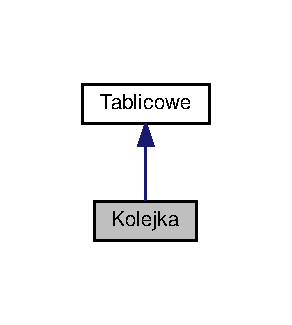
\includegraphics[width=140pt]{class_kolejka__inherit__graph}
\end{center}
\end{figure}


Diagram współpracy dla Kolejka\-:\nopagebreak
\begin{figure}[H]
\begin{center}
\leavevmode
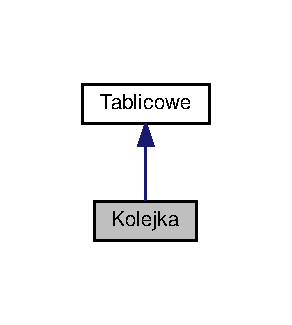
\includegraphics[width=140pt]{class_kolejka__coll__graph}
\end{center}
\end{figure}
\subsection*{Metody publiczne}
\begin{DoxyCompactItemize}
\item 
\hyperlink{class_kolejka_a37c886fdc73dce62b04da0381dec5484}{Kolejka} ()
\begin{DoxyCompactList}\small\item\em Konstruktor obiektu \hyperlink{class_kolejka}{Kolejka}. Tworzy kolejke o domyslnym rozmiarze rownym 8. \end{DoxyCompactList}\item 
\hyperlink{class_kolejka_ac942cc97bf0d2c30d11611c406acc5a8}{Kolejka} (long \-\_\-size)
\begin{DoxyCompactList}\small\item\em Konstruktor parametryczny obiektu \hyperlink{class_kolejka}{Kolejka}. Tworzy kolejke o zadanym rozmiarze rownym \-\_\-size. \end{DoxyCompactList}\item 
\hyperlink{class_kolejka_a352f86ff08cd47be6c35c60bb0f873a6}{$\sim$\-Kolejka} ()
\begin{DoxyCompactList}\small\item\em Destruktor obiektu \hyperlink{class_kolejka}{Kolejka}. \end{DoxyCompactList}\item 
void \hyperlink{class_kolejka_a8f3b0111e85f517d9eadb8ce996d4471}{enqueue} (int \-\_\-elem)
\begin{DoxyCompactList}\small\item\em Metoda dodawnia elementu. Metoda sluzy do dodawania elementu do kolejki. \end{DoxyCompactList}\item 
int \hyperlink{class_kolejka_af23261614bcf242a1934a99688a2debc}{dequeue} ()
\begin{DoxyCompactList}\small\item\em Metoda usuwania elementu. Metoda sluzy do usuwania elementu z kolejki. \end{DoxyCompactList}\end{DoxyCompactItemize}
\subsection*{Metody prywatne}
\begin{DoxyCompactItemize}
\item 
void \hyperlink{class_kolejka_ab4f51f0ec7fef36a85af6cfd1c257427}{increase} ()
\begin{DoxyCompactList}\small\item\em Metoda powiekszania kolejki. Metoda ta zwieksza ilosc pol w kolejce dwukrotnie. \end{DoxyCompactList}\item 
int \hyperlink{class_kolejka_acff09ebfbec69b06c91203bab30d815d}{decrease} ()
\begin{DoxyCompactList}\small\item\em Metoda pomniejszania kolejki. Metoda ta odejmuje od kolejki jedno pole. \end{DoxyCompactList}\end{DoxyCompactItemize}
\subsection*{Dodatkowe Dziedziczone Składowe}


\subsection{Opis szczegółowy}


Definicja w linii 10 pliku kolejka.\-hh.



\subsection{Dokumentacja konstruktora i destruktora}
\hypertarget{class_kolejka_a37c886fdc73dce62b04da0381dec5484}{\index{Kolejka@{Kolejka}!Kolejka@{Kolejka}}
\index{Kolejka@{Kolejka}!Kolejka@{Kolejka}}
\subsubsection[{Kolejka}]{\setlength{\rightskip}{0pt plus 5cm}Kolejka\-::\-Kolejka (
\begin{DoxyParamCaption}
{}
\end{DoxyParamCaption}
)}}\label{class_kolejka_a37c886fdc73dce62b04da0381dec5484}


Definicja w linii 7 pliku kolejka.\-cpp.

\hypertarget{class_kolejka_ac942cc97bf0d2c30d11611c406acc5a8}{\index{Kolejka@{Kolejka}!Kolejka@{Kolejka}}
\index{Kolejka@{Kolejka}!Kolejka@{Kolejka}}
\subsubsection[{Kolejka}]{\setlength{\rightskip}{0pt plus 5cm}Kolejka\-::\-Kolejka (
\begin{DoxyParamCaption}
\item[{long}]{\-\_\-size}
\end{DoxyParamCaption}
)}}\label{class_kolejka_ac942cc97bf0d2c30d11611c406acc5a8}

\begin{DoxyParams}[1]{Parametry}
\mbox{\tt in}  & {\em \-\_\-size} & -\/ startowy rozmiar struktury. \\
\hline
\end{DoxyParams}


Definicja w linii 17 pliku kolejka.\-cpp.

\hypertarget{class_kolejka_a352f86ff08cd47be6c35c60bb0f873a6}{\index{Kolejka@{Kolejka}!$\sim$\-Kolejka@{$\sim$\-Kolejka}}
\index{$\sim$\-Kolejka@{$\sim$\-Kolejka}!Kolejka@{Kolejka}}
\subsubsection[{$\sim$\-Kolejka}]{\setlength{\rightskip}{0pt plus 5cm}Kolejka\-::$\sim$\-Kolejka (
\begin{DoxyParamCaption}
{}
\end{DoxyParamCaption}
)}}\label{class_kolejka_a352f86ff08cd47be6c35c60bb0f873a6}


Definicja w linii 27 pliku kolejka.\-cpp.



\subsection{Dokumentacja funkcji składowych}
\hypertarget{class_kolejka_acff09ebfbec69b06c91203bab30d815d}{\index{Kolejka@{Kolejka}!decrease@{decrease}}
\index{decrease@{decrease}!Kolejka@{Kolejka}}
\subsubsection[{decrease}]{\setlength{\rightskip}{0pt plus 5cm}int Kolejka\-::decrease (
\begin{DoxyParamCaption}
{}
\end{DoxyParamCaption}
)\hspace{0.3cm}{\ttfamily [private]}}}\label{class_kolejka_acff09ebfbec69b06c91203bab30d815d}


Definicja w linii 45 pliku kolejka.\-cpp.



Oto graf wywoływań tej funkcji\-:\nopagebreak
\begin{figure}[H]
\begin{center}
\leavevmode
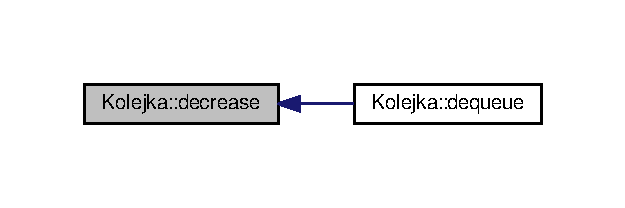
\includegraphics[width=300pt]{class_kolejka_acff09ebfbec69b06c91203bab30d815d_icgraph}
\end{center}
\end{figure}


\hypertarget{class_kolejka_af23261614bcf242a1934a99688a2debc}{\index{Kolejka@{Kolejka}!dequeue@{dequeue}}
\index{dequeue@{dequeue}!Kolejka@{Kolejka}}
\subsubsection[{dequeue}]{\setlength{\rightskip}{0pt plus 5cm}int Kolejka\-::dequeue (
\begin{DoxyParamCaption}
{}
\end{DoxyParamCaption}
)}}\label{class_kolejka_af23261614bcf242a1934a99688a2debc}
\begin{DoxyReturn}{Zwraca}
usuwany element. 
\end{DoxyReturn}


Definicja w linii 69 pliku kolejka.\-cpp.



Oto graf wywołań dla tej funkcji\-:\nopagebreak
\begin{figure}[H]
\begin{center}
\leavevmode
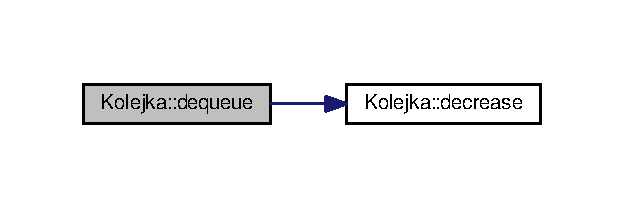
\includegraphics[width=300pt]{class_kolejka_af23261614bcf242a1934a99688a2debc_cgraph}
\end{center}
\end{figure}


\hypertarget{class_kolejka_a8f3b0111e85f517d9eadb8ce996d4471}{\index{Kolejka@{Kolejka}!enqueue@{enqueue}}
\index{enqueue@{enqueue}!Kolejka@{Kolejka}}
\subsubsection[{enqueue}]{\setlength{\rightskip}{0pt plus 5cm}void Kolejka\-::enqueue (
\begin{DoxyParamCaption}
\item[{int}]{\-\_\-elem}
\end{DoxyParamCaption}
)}}\label{class_kolejka_a8f3b0111e85f517d9eadb8ce996d4471}

\begin{DoxyParams}[1]{Parametry}
\mbox{\tt in}  & {\em \-\_\-elem} & -\/ dodawany element. \\
\hline
\end{DoxyParams}


Definicja w linii 60 pliku kolejka.\-cpp.



Oto graf wywołań dla tej funkcji\-:\nopagebreak
\begin{figure}[H]
\begin{center}
\leavevmode
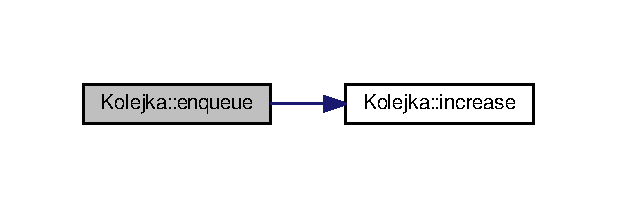
\includegraphics[width=296pt]{class_kolejka_a8f3b0111e85f517d9eadb8ce996d4471_cgraph}
\end{center}
\end{figure}


\hypertarget{class_kolejka_ab4f51f0ec7fef36a85af6cfd1c257427}{\index{Kolejka@{Kolejka}!increase@{increase}}
\index{increase@{increase}!Kolejka@{Kolejka}}
\subsubsection[{increase}]{\setlength{\rightskip}{0pt plus 5cm}void Kolejka\-::increase (
\begin{DoxyParamCaption}
{}
\end{DoxyParamCaption}
)\hspace{0.3cm}{\ttfamily [private]}}}\label{class_kolejka_ab4f51f0ec7fef36a85af6cfd1c257427}


Definicja w linii 33 pliku kolejka.\-cpp.



Oto graf wywoływań tej funkcji\-:\nopagebreak
\begin{figure}[H]
\begin{center}
\leavevmode
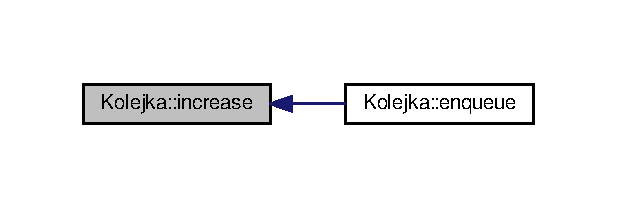
\includegraphics[width=296pt]{class_kolejka_ab4f51f0ec7fef36a85af6cfd1c257427_icgraph}
\end{center}
\end{figure}




Dokumentacja dla tej klasy została wygenerowana z plików\-:\begin{DoxyCompactItemize}
\item 
\hyperlink{kolejka_8hh}{kolejka.\-hh}\item 
\hyperlink{kolejka_8cpp}{kolejka.\-cpp}\end{DoxyCompactItemize}

\hypertarget{struct_lista_1_1_komorka}{\section{Dokumentacja struktury Lista\-:\-:Komorka}
\label{struct_lista_1_1_komorka}\index{Lista\-::\-Komorka@{Lista\-::\-Komorka}}
}


Struktura \hyperlink{struct_lista_1_1_komorka}{Komorka}. Obiekt tego typu reprezentuje pojedyncza komorke wraz ze wskaznikiem na nastepna komorke listy.  




Diagram współpracy dla Lista\-:\-:Komorka\-:\nopagebreak
\begin{figure}[H]
\begin{center}
\leavevmode
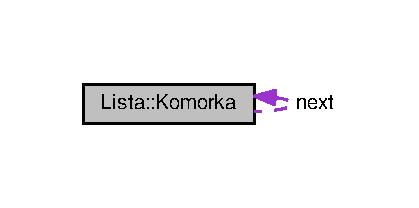
\includegraphics[width=201pt]{struct_lista_1_1_komorka__coll__graph}
\end{center}
\end{figure}
\subsection*{Metody publiczne}
\begin{DoxyCompactItemize}
\item 
\hyperlink{struct_lista_1_1_komorka_a1843c3c4ae9752cea90cfa21076f3e9c}{Komorka} (int \-\_\-elem)
\begin{DoxyCompactList}\small\item\em Konstruktor paramteryczny obiektu \hyperlink{struct_lista_1_1_komorka}{Komorka}. \end{DoxyCompactList}\item 
\hyperlink{struct_lista_1_1_komorka_a91f3a7f9bd8ebe05fa0821e1d989c506}{$\sim$\-Komorka} ()
\end{DoxyCompactItemize}
\subsection*{Atrybuty publiczne}
\begin{DoxyCompactItemize}
\item 
int \hyperlink{struct_lista_1_1_komorka_aeb683e1dce8a8c096cc54a6645137411}{elem}
\begin{DoxyCompactList}\small\item\em Wartosc elementu w pojedynczej komorce. \end{DoxyCompactList}\item 
\hyperlink{struct_lista_1_1_komorka}{Komorka} $\ast$ \hyperlink{struct_lista_1_1_komorka_aa04e9d2ed0260f2adbff6855f7bcd77e}{next}
\begin{DoxyCompactList}\small\item\em Wskaznik na nastepna komorke listy. \end{DoxyCompactList}\end{DoxyCompactItemize}


\subsection{Opis szczegółowy}


Definicja w linii 16 pliku lista.\-hh.



\subsection{Dokumentacja konstruktora i destruktora}
\hypertarget{struct_lista_1_1_komorka_a1843c3c4ae9752cea90cfa21076f3e9c}{\index{Lista\-::\-Komorka@{Lista\-::\-Komorka}!Komorka@{Komorka}}
\index{Komorka@{Komorka}!Lista::Komorka@{Lista\-::\-Komorka}}
\subsubsection[{Komorka}]{\setlength{\rightskip}{0pt plus 5cm}Lista\-::\-Komorka\-::\-Komorka (
\begin{DoxyParamCaption}
\item[{int}]{\-\_\-elem}
\end{DoxyParamCaption}
)\hspace{0.3cm}{\ttfamily [inline]}}}\label{struct_lista_1_1_komorka_a1843c3c4ae9752cea90cfa21076f3e9c}

\begin{DoxyParams}[1]{Parametry}
\mbox{\tt in}  & {\em \-\_\-elem} & -\/ wartosc przechowywanego elementu. \\
\hline
\end{DoxyParams}


Definicja w linii 29 pliku lista.\-hh.

\hypertarget{struct_lista_1_1_komorka_a91f3a7f9bd8ebe05fa0821e1d989c506}{\index{Lista\-::\-Komorka@{Lista\-::\-Komorka}!$\sim$\-Komorka@{$\sim$\-Komorka}}
\index{$\sim$\-Komorka@{$\sim$\-Komorka}!Lista::Komorka@{Lista\-::\-Komorka}}
\subsubsection[{$\sim$\-Komorka}]{\setlength{\rightskip}{0pt plus 5cm}Lista\-::\-Komorka\-::$\sim$\-Komorka (
\begin{DoxyParamCaption}
{}
\end{DoxyParamCaption}
)\hspace{0.3cm}{\ttfamily [inline]}}}\label{struct_lista_1_1_komorka_a91f3a7f9bd8ebe05fa0821e1d989c506}


Definicja w linii 33 pliku lista.\-hh.



\subsection{Dokumentacja atrybutów składowych}
\hypertarget{struct_lista_1_1_komorka_aeb683e1dce8a8c096cc54a6645137411}{\index{Lista\-::\-Komorka@{Lista\-::\-Komorka}!elem@{elem}}
\index{elem@{elem}!Lista::Komorka@{Lista\-::\-Komorka}}
\subsubsection[{elem}]{\setlength{\rightskip}{0pt plus 5cm}int Lista\-::\-Komorka\-::elem}}\label{struct_lista_1_1_komorka_aeb683e1dce8a8c096cc54a6645137411}


Definicja w linii 20 pliku lista.\-hh.

\hypertarget{struct_lista_1_1_komorka_aa04e9d2ed0260f2adbff6855f7bcd77e}{\index{Lista\-::\-Komorka@{Lista\-::\-Komorka}!next@{next}}
\index{next@{next}!Lista::Komorka@{Lista\-::\-Komorka}}
\subsubsection[{next}]{\setlength{\rightskip}{0pt plus 5cm}{\bf Komorka}$\ast$ Lista\-::\-Komorka\-::next}}\label{struct_lista_1_1_komorka_aa04e9d2ed0260f2adbff6855f7bcd77e}


Definicja w linii 24 pliku lista.\-hh.



Dokumentacja dla tej struktury została wygenerowana z pliku\-:\begin{DoxyCompactItemize}
\item 
\hyperlink{lista_8hh}{lista.\-hh}\end{DoxyCompactItemize}

\hypertarget{class_lista}{\section{Dokumentacja klasy Lista}
\label{class_lista}\index{Lista@{Lista}}
}


Klasa \hyperlink{class_lista}{Lista} modelujaca strukture danych typu lista. Obiekt tego typu reprezentuje strukture danych typu lista wraz z operacjami mozliwymi do wykonania na tej strukturze.  




{\ttfamily \#include $<$lista.\-hh$>$}



Diagram współpracy dla Lista\-:\nopagebreak
\begin{figure}[H]
\begin{center}
\leavevmode
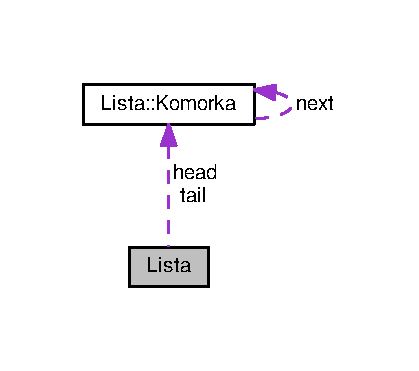
\includegraphics[width=201pt]{class_lista__coll__graph}
\end{center}
\end{figure}
\subsection*{Komponenty}
\begin{DoxyCompactItemize}
\item 
struct \hyperlink{struct_lista_1_1_komorka}{Komorka}
\begin{DoxyCompactList}\small\item\em Struktura \hyperlink{struct_lista_1_1_komorka}{Komorka}. Obiekt tego typu reprezentuje pojedyncza komorke wraz ze wskaznikiem na nastepna komorke listy. \end{DoxyCompactList}\end{DoxyCompactItemize}
\subsection*{Metody publiczne}
\begin{DoxyCompactItemize}
\item 
\hyperlink{class_lista_a1f668b36909182ef1360b48503529a31}{Lista} ()
\begin{DoxyCompactList}\small\item\em Konstruktor obiektu \hyperlink{class_lista}{Lista}. \end{DoxyCompactList}\item 
\hyperlink{class_lista_a4d7394b2728a00ad8404965b2e15d096}{$\sim$\-Lista} ()
\begin{DoxyCompactList}\small\item\em Destruktor obiektu \hyperlink{class_lista}{Lista}. \end{DoxyCompactList}\item 
void \hyperlink{class_lista_acec8ac807da644d8250c3c6043a208e1}{insert} (int \-\_\-elem)
\begin{DoxyCompactList}\small\item\em Metoda dodawnia elementu. Metoda sluzy do dodawania elementu do konca listy. \end{DoxyCompactList}\item 
void \hyperlink{class_lista_aa30ec43a5b51a0e37ffe8f098c5dcaa8}{remove} (int \-\_\-f)
\begin{DoxyCompactList}\small\item\em Metoda usuwania elementu. Metoda sluzy do usuwania elementu o wskazanym indeksie. \end{DoxyCompactList}\end{DoxyCompactItemize}
\subsection*{Atrybuty prywatne}
\begin{DoxyCompactItemize}
\item 
\hyperlink{struct_lista_1_1_komorka}{Komorka} $\ast$ \hyperlink{class_lista_aeba20505030183d334971bd44c3c8b95}{head}
\begin{DoxyCompactList}\small\item\em Wskaznik na poczatek listy. \end{DoxyCompactList}\item 
\hyperlink{struct_lista_1_1_komorka}{Komorka} $\ast$ \hyperlink{class_lista_a7d42e5f99e945d97c29d6f764f71f4e7}{tail}
\begin{DoxyCompactList}\small\item\em Wskaznik na koniec listy. \end{DoxyCompactList}\end{DoxyCompactItemize}


\subsection{Opis szczegółowy}


Definicja w linii 9 pliku lista.\-hh.



\subsection{Dokumentacja konstruktora i destruktora}
\hypertarget{class_lista_a1f668b36909182ef1360b48503529a31}{\index{Lista@{Lista}!Lista@{Lista}}
\index{Lista@{Lista}!Lista@{Lista}}
\subsubsection[{Lista}]{\setlength{\rightskip}{0pt plus 5cm}Lista\-::\-Lista (
\begin{DoxyParamCaption}
{}
\end{DoxyParamCaption}
)\hspace{0.3cm}{\ttfamily [inline]}}}\label{class_lista_a1f668b36909182ef1360b48503529a31}


Definicja w linii 49 pliku lista.\-hh.

\hypertarget{class_lista_a4d7394b2728a00ad8404965b2e15d096}{\index{Lista@{Lista}!$\sim$\-Lista@{$\sim$\-Lista}}
\index{$\sim$\-Lista@{$\sim$\-Lista}!Lista@{Lista}}
\subsubsection[{$\sim$\-Lista}]{\setlength{\rightskip}{0pt plus 5cm}Lista\-::$\sim$\-Lista (
\begin{DoxyParamCaption}
{}
\end{DoxyParamCaption}
)\hspace{0.3cm}{\ttfamily [inline]}}}\label{class_lista_a4d7394b2728a00ad8404965b2e15d096}


Definicja w linii 54 pliku lista.\-hh.



\subsection{Dokumentacja funkcji składowych}
\hypertarget{class_lista_acec8ac807da644d8250c3c6043a208e1}{\index{Lista@{Lista}!insert@{insert}}
\index{insert@{insert}!Lista@{Lista}}
\subsubsection[{insert}]{\setlength{\rightskip}{0pt plus 5cm}void Lista\-::insert (
\begin{DoxyParamCaption}
\item[{int}]{\-\_\-elem}
\end{DoxyParamCaption}
)}}\label{class_lista_acec8ac807da644d8250c3c6043a208e1}

\begin{DoxyParams}[1]{Parametry}
\mbox{\tt in}  & {\em \-\_\-elem} & -\/ dodawany element. \\
\hline
\end{DoxyParams}


Definicja w linii 5 pliku lista.\-cpp.



Oto graf wywoływań tej funkcji\-:\nopagebreak
\begin{figure}[H]
\begin{center}
\leavevmode
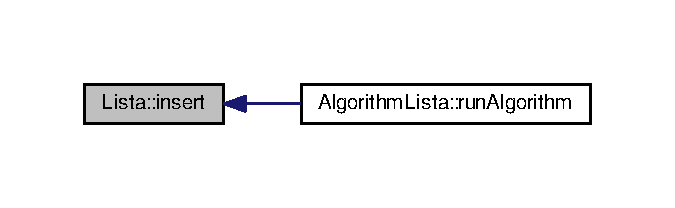
\includegraphics[width=324pt]{class_lista_acec8ac807da644d8250c3c6043a208e1_icgraph}
\end{center}
\end{figure}


\hypertarget{class_lista_aa30ec43a5b51a0e37ffe8f098c5dcaa8}{\index{Lista@{Lista}!remove@{remove}}
\index{remove@{remove}!Lista@{Lista}}
\subsubsection[{remove}]{\setlength{\rightskip}{0pt plus 5cm}void Lista\-::remove (
\begin{DoxyParamCaption}
\item[{int}]{\-\_\-f}
\end{DoxyParamCaption}
)}}\label{class_lista_aa30ec43a5b51a0e37ffe8f098c5dcaa8}

\begin{DoxyParams}[1]{Parametry}
\mbox{\tt in}  & {\em \-\_\-f} & -\/ indeks elementu do usuniecia. \\
\hline
\end{DoxyParams}


Definicja w linii 19 pliku lista.\-cpp.



\subsection{Dokumentacja atrybutów składowych}
\hypertarget{class_lista_aeba20505030183d334971bd44c3c8b95}{\index{Lista@{Lista}!head@{head}}
\index{head@{head}!Lista@{Lista}}
\subsubsection[{head}]{\setlength{\rightskip}{0pt plus 5cm}{\bf Komorka}$\ast$ Lista\-::head\hspace{0.3cm}{\ttfamily [private]}}}\label{class_lista_aeba20505030183d334971bd44c3c8b95}


Definicja w linii 38 pliku lista.\-hh.

\hypertarget{class_lista_a7d42e5f99e945d97c29d6f764f71f4e7}{\index{Lista@{Lista}!tail@{tail}}
\index{tail@{tail}!Lista@{Lista}}
\subsubsection[{tail}]{\setlength{\rightskip}{0pt plus 5cm}{\bf Komorka}$\ast$ Lista\-::tail\hspace{0.3cm}{\ttfamily [private]}}}\label{class_lista_a7d42e5f99e945d97c29d6f764f71f4e7}


Definicja w linii 42 pliku lista.\-hh.



Dokumentacja dla tej klasy została wygenerowana z plików\-:\begin{DoxyCompactItemize}
\item 
\hyperlink{lista_8hh}{lista.\-hh}\item 
\hyperlink{lista_8cpp}{lista.\-cpp}\end{DoxyCompactItemize}

\hypertarget{class_stos}{\section{Dokumentacja klasy Stos}
\label{class_stos}\index{Stos@{Stos}}
}


Klasa \hyperlink{class_stos}{Stos} modelujaca strukture danych typu stos. Obiekt tego typu reprezentuje strukture danych typu stos wraz z operacjami mozliwymi do wykonania na tej strukturze.  




{\ttfamily \#include $<$stos.\-hh$>$}

\subsection*{Metody publiczne}
\begin{DoxyCompactItemize}
\item 
\hyperlink{class_stos_a1de3b50386d5dfb56ddece17d0ea2389}{Stos} ()
\begin{DoxyCompactList}\small\item\em Konstruktor obiektu \hyperlink{class_stos}{Stos}. \end{DoxyCompactList}\item 
\hyperlink{class_stos_a6606affc11eed2b059b8caf287ffca25}{Stos} (long \-\_\-size)
\begin{DoxyCompactList}\small\item\em Konstruktor parametryczny obiektu \hyperlink{class_stos}{Stos}. \end{DoxyCompactList}\item 
\hyperlink{class_stos_af9a198e2540e18adcc0b5259105fd78e}{$\sim$\-Stos} ()
\begin{DoxyCompactList}\small\item\em Destruktor obiektu \hyperlink{class_stos}{Stos}. \end{DoxyCompactList}\item 
void \hyperlink{class_stos_afd5802e405946328cccca3eed676b493}{push} (int \-\_\-elem)
\begin{DoxyCompactList}\small\item\em Metoda dodawnia elementu. Metoda sluzy do dodawania elementu do stosu. \end{DoxyCompactList}\item 
int \hyperlink{class_stos_aabb14b8a389c55da6e2b50fbb179ed56}{pop} ()
\begin{DoxyCompactList}\small\item\em Metoda usuwania elementu. Metoda sluzy do usuwania elementu ze stosu. \end{DoxyCompactList}\end{DoxyCompactItemize}
\subsection*{Metody prywatne}
\begin{DoxyCompactItemize}
\item 
void \hyperlink{class_stos_aaf6e4717d1983c5351c9f5e9797368d3}{increase} ()
\begin{DoxyCompactList}\small\item\em Metoda powiekszania stosu. Metoda ta dodaje do stosu 8 kolejnych wolnych pol. \end{DoxyCompactList}\item 
int \hyperlink{class_stos_a1054dda0231b2516b6a04298801c0b27}{decrease} ()
\begin{DoxyCompactList}\small\item\em Metoda pomniejszania stosu. Metoda ta odejmuje od stosu jedno pole. \end{DoxyCompactList}\end{DoxyCompactItemize}
\subsection*{Atrybuty prywatne}
\begin{DoxyCompactItemize}
\item 
int $\ast$ \hyperlink{class_stos_abcb666dd5a69fe50228595dc8ac4160a}{tab}
\begin{DoxyCompactList}\small\item\em Wskaznik na tablice elementow stosu. \end{DoxyCompactList}\item 
long \hyperlink{class_stos_a07ba18a24f8f0dbd9144406d15bcd342}{size}
\begin{DoxyCompactList}\small\item\em Rozmiar stosu. \end{DoxyCompactList}\item 
long \hyperlink{class_stos_ae0623cdf9b6725e38da86b74972d61ba}{last}
\begin{DoxyCompactList}\small\item\em Indeks ostatniego wolnego pola. \end{DoxyCompactList}\end{DoxyCompactItemize}


\subsection{Opis szczegółowy}


Definicja w linii 9 pliku stos.\-hh.



\subsection{Dokumentacja konstruktora i destruktora}
\hypertarget{class_stos_a1de3b50386d5dfb56ddece17d0ea2389}{\index{Stos@{Stos}!Stos@{Stos}}
\index{Stos@{Stos}!Stos@{Stos}}
\subsubsection[{Stos}]{\setlength{\rightskip}{0pt plus 5cm}Stos\-::\-Stos (
\begin{DoxyParamCaption}
{}
\end{DoxyParamCaption}
)}}\label{class_stos_a1de3b50386d5dfb56ddece17d0ea2389}


Definicja w linii 6 pliku stos.\-cpp.

\hypertarget{class_stos_a6606affc11eed2b059b8caf287ffca25}{\index{Stos@{Stos}!Stos@{Stos}}
\index{Stos@{Stos}!Stos@{Stos}}
\subsubsection[{Stos}]{\setlength{\rightskip}{0pt plus 5cm}Stos\-::\-Stos (
\begin{DoxyParamCaption}
\item[{long}]{\-\_\-size}
\end{DoxyParamCaption}
)}}\label{class_stos_a6606affc11eed2b059b8caf287ffca25}

\begin{DoxyParams}[1]{Parametry}
\mbox{\tt in}  & {\em \-\_\-size} & -\/ rozmiar tworzonego stosu. \\
\hline
\end{DoxyParams}


Definicja w linii 17 pliku stos.\-cpp.

\hypertarget{class_stos_af9a198e2540e18adcc0b5259105fd78e}{\index{Stos@{Stos}!$\sim$\-Stos@{$\sim$\-Stos}}
\index{$\sim$\-Stos@{$\sim$\-Stos}!Stos@{Stos}}
\subsubsection[{$\sim$\-Stos}]{\setlength{\rightskip}{0pt plus 5cm}Stos\-::$\sim$\-Stos (
\begin{DoxyParamCaption}
{}
\end{DoxyParamCaption}
)}}\label{class_stos_af9a198e2540e18adcc0b5259105fd78e}


Definicja w linii 28 pliku stos.\-cpp.



\subsection{Dokumentacja funkcji składowych}
\hypertarget{class_stos_a1054dda0231b2516b6a04298801c0b27}{\index{Stos@{Stos}!decrease@{decrease}}
\index{decrease@{decrease}!Stos@{Stos}}
\subsubsection[{decrease}]{\setlength{\rightskip}{0pt plus 5cm}int Stos\-::decrease (
\begin{DoxyParamCaption}
{}
\end{DoxyParamCaption}
)\hspace{0.3cm}{\ttfamily [private]}}}\label{class_stos_a1054dda0231b2516b6a04298801c0b27}


Definicja w linii 63 pliku stos.\-cpp.



Oto graf wywoływań tej funkcji\-:\nopagebreak
\begin{figure}[H]
\begin{center}
\leavevmode
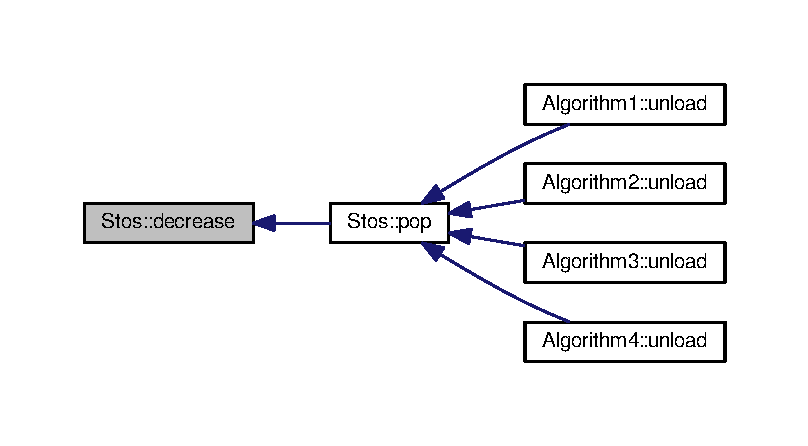
\includegraphics[width=256pt]{class_stos_a1054dda0231b2516b6a04298801c0b27_icgraph}
\end{center}
\end{figure}


\hypertarget{class_stos_aaf6e4717d1983c5351c9f5e9797368d3}{\index{Stos@{Stos}!increase@{increase}}
\index{increase@{increase}!Stos@{Stos}}
\subsubsection[{increase}]{\setlength{\rightskip}{0pt plus 5cm}void Stos\-::increase (
\begin{DoxyParamCaption}
{}
\end{DoxyParamCaption}
)\hspace{0.3cm}{\ttfamily [private]}}}\label{class_stos_aaf6e4717d1983c5351c9f5e9797368d3}


Definicja w linii 51 pliku stos.\-cpp.



Oto graf wywoływań tej funkcji\-:\nopagebreak
\begin{figure}[H]
\begin{center}
\leavevmode
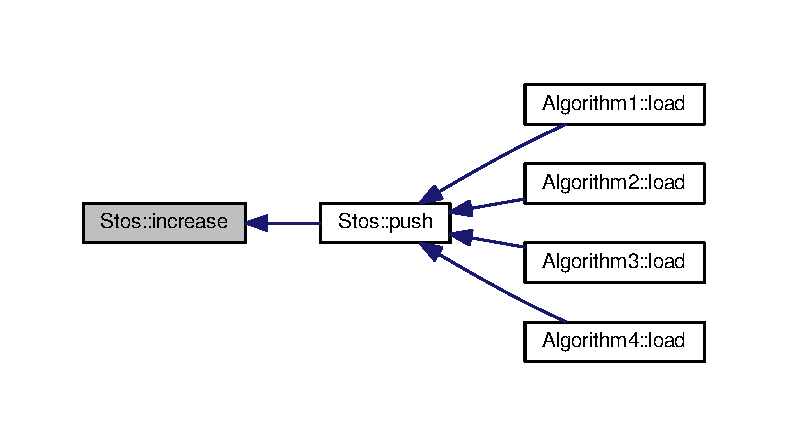
\includegraphics[width=350pt]{class_stos_aaf6e4717d1983c5351c9f5e9797368d3_icgraph}
\end{center}
\end{figure}


\hypertarget{class_stos_aabb14b8a389c55da6e2b50fbb179ed56}{\index{Stos@{Stos}!pop@{pop}}
\index{pop@{pop}!Stos@{Stos}}
\subsubsection[{pop}]{\setlength{\rightskip}{0pt plus 5cm}int Stos\-::pop (
\begin{DoxyParamCaption}
{}
\end{DoxyParamCaption}
)}}\label{class_stos_aabb14b8a389c55da6e2b50fbb179ed56}
\begin{DoxyReturn}{Zwraca}
-\/ usuwany element. 
\end{DoxyReturn}


Definicja w linii 43 pliku stos.\-cpp.



Oto graf wywołań dla tej funkcji\-:\nopagebreak
\begin{figure}[H]
\begin{center}
\leavevmode
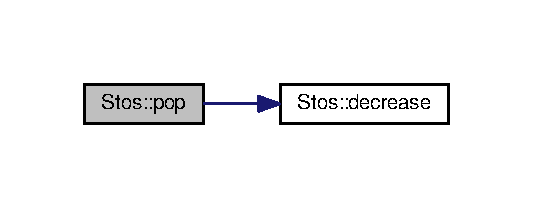
\includegraphics[width=256pt]{class_stos_aabb14b8a389c55da6e2b50fbb179ed56_cgraph}
\end{center}
\end{figure}


\hypertarget{class_stos_afd5802e405946328cccca3eed676b493}{\index{Stos@{Stos}!push@{push}}
\index{push@{push}!Stos@{Stos}}
\subsubsection[{push}]{\setlength{\rightskip}{0pt plus 5cm}void Stos\-::push (
\begin{DoxyParamCaption}
\item[{int}]{\-\_\-elem}
\end{DoxyParamCaption}
)}}\label{class_stos_afd5802e405946328cccca3eed676b493}

\begin{DoxyParams}[1]{Parametry}
\mbox{\tt in}  & {\em \-\_\-elem} & -\/ dodawany element. \\
\hline
\end{DoxyParams}


Definicja w linii 34 pliku stos.\-cpp.



Oto graf wywołań dla tej funkcji\-:\nopagebreak
\begin{figure}[H]
\begin{center}
\leavevmode
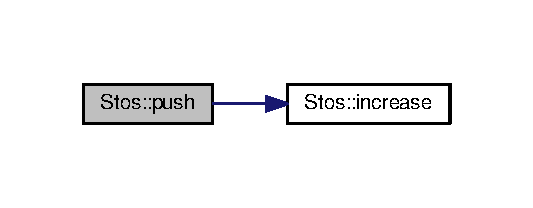
\includegraphics[width=256pt]{class_stos_afd5802e405946328cccca3eed676b493_cgraph}
\end{center}
\end{figure}




Oto graf wywoływań tej funkcji\-:\nopagebreak
\begin{figure}[H]
\begin{center}
\leavevmode
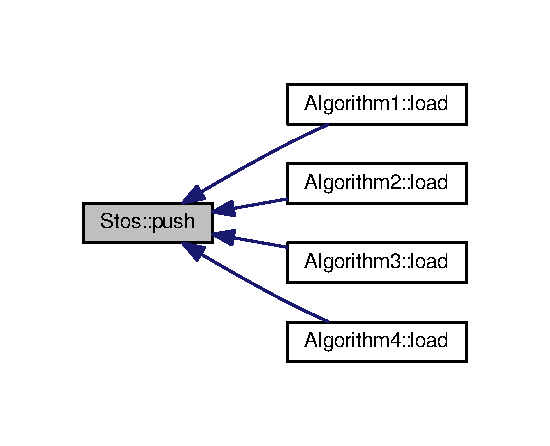
\includegraphics[width=316pt]{class_stos_afd5802e405946328cccca3eed676b493_icgraph}
\end{center}
\end{figure}




\subsection{Dokumentacja atrybutów składowych}
\hypertarget{class_stos_ae0623cdf9b6725e38da86b74972d61ba}{\index{Stos@{Stos}!last@{last}}
\index{last@{last}!Stos@{Stos}}
\subsubsection[{last}]{\setlength{\rightskip}{0pt plus 5cm}long Stos\-::last\hspace{0.3cm}{\ttfamily [private]}}}\label{class_stos_ae0623cdf9b6725e38da86b74972d61ba}


Definicja w linii 22 pliku stos.\-hh.

\hypertarget{class_stos_a07ba18a24f8f0dbd9144406d15bcd342}{\index{Stos@{Stos}!size@{size}}
\index{size@{size}!Stos@{Stos}}
\subsubsection[{size}]{\setlength{\rightskip}{0pt plus 5cm}long Stos\-::size\hspace{0.3cm}{\ttfamily [private]}}}\label{class_stos_a07ba18a24f8f0dbd9144406d15bcd342}


Definicja w linii 18 pliku stos.\-hh.

\hypertarget{class_stos_abcb666dd5a69fe50228595dc8ac4160a}{\index{Stos@{Stos}!tab@{tab}}
\index{tab@{tab}!Stos@{Stos}}
\subsubsection[{tab}]{\setlength{\rightskip}{0pt plus 5cm}int$\ast$ Stos\-::tab\hspace{0.3cm}{\ttfamily [private]}}}\label{class_stos_abcb666dd5a69fe50228595dc8ac4160a}


Definicja w linii 14 pliku stos.\-hh.



Dokumentacja dla tej klasy została wygenerowana z plików\-:\begin{DoxyCompactItemize}
\item 
\hyperlink{stos_8hh}{stos.\-hh}\item 
\hyperlink{stos_8cpp}{stos.\-cpp}\end{DoxyCompactItemize}

\hypertarget{class_tab_lista}{\section{Dokumentacja klasy Tab\-Lista}
\label{class_tab_lista}\index{Tab\-Lista@{Tab\-Lista}}
}


Klasa \hyperlink{class_tab_lista}{Tab\-Lista} modelujaca strukture danych typu lista. Obiekt tego typu reprezentuje strukture danych typu lista zaimplementowana na tablicy dynamicznej. Obiekt zawiera rowniez podstowe metody listy.  




{\ttfamily \#include $<$tab\-\_\-lista.\-hh$>$}

\subsection*{Metody publiczne}
\begin{DoxyCompactItemize}
\item 
\hyperlink{class_tab_lista_ad3bfa98306e98b4e5bb7ff524e72078c}{Tab\-Lista} ()
\begin{DoxyCompactList}\small\item\em Konstruktor obiektu \hyperlink{class_tab_lista}{Tab\-Lista}. \end{DoxyCompactList}\item 
\hyperlink{class_tab_lista_a95d23d52e0af187351b3fc1022ae4839}{Tab\-Lista} (long \-\_\-size)
\begin{DoxyCompactList}\small\item\em Konstruktor parametryczny obiektu \hyperlink{class_tab_lista}{Tab\-Lista}. \end{DoxyCompactList}\item 
\hyperlink{class_tab_lista_a0b4a808158b370bbc5785ceef760a273}{$\sim$\-Tab\-Lista} ()
\begin{DoxyCompactList}\small\item\em Destruktor obiektu \hyperlink{class_tab_lista}{Tab\-Lista}. \end{DoxyCompactList}\item 
void \hyperlink{class_tab_lista_a7bd3e5f62a81bfd3813ad874e8a9c059}{insert} (int \-\_\-elem)
\begin{DoxyCompactList}\small\item\em Metoda dodawnia elementu. Metoda sluzy do dodawania elementu do konca listy. \end{DoxyCompactList}\item 
int \hyperlink{class_tab_lista_aae59a3eafbbd7424a952badb26410a5e}{remove} (int \-\_\-f)
\begin{DoxyCompactList}\small\item\em Metoda usuwania elementu. Metoda sluzy do usuwania elementu o wskazanym indeksie. \end{DoxyCompactList}\end{DoxyCompactItemize}
\subsection*{Metody prywatne}
\begin{DoxyCompactItemize}
\item 
void \hyperlink{class_tab_lista_a9ae6a784d488c8b9885ccbc945225f9e}{increase} ()
\begin{DoxyCompactList}\small\item\em Metoda powiekszania listy tablicowe. Metoda ta dodaje do listy 8 kolejnych wolnych pol. \end{DoxyCompactList}\end{DoxyCompactItemize}
\subsection*{Atrybuty prywatne}
\begin{DoxyCompactItemize}
\item 
int $\ast$ \hyperlink{class_tab_lista_a06f658ed62f3db852813e90dcc5876a5}{tab}
\begin{DoxyCompactList}\small\item\em Wskaznik na tablice elementow listy. \end{DoxyCompactList}\item 
long \hyperlink{class_tab_lista_aa3c6d623be318ec8410fa447281380da}{size}
\begin{DoxyCompactList}\small\item\em Rozmiar listy. \end{DoxyCompactList}\item 
long \hyperlink{class_tab_lista_ac7413a3d41c2c2e57fa92e055fc2e5b3}{last}
\begin{DoxyCompactList}\small\item\em Wskaznik na ostatni wolny element. \end{DoxyCompactList}\end{DoxyCompactItemize}


\subsection{Opis szczegółowy}


Definicja w linii 10 pliku tab\-\_\-lista.\-hh.



\subsection{Dokumentacja konstruktora i destruktora}
\hypertarget{class_tab_lista_ad3bfa98306e98b4e5bb7ff524e72078c}{\index{Tab\-Lista@{Tab\-Lista}!Tab\-Lista@{Tab\-Lista}}
\index{Tab\-Lista@{Tab\-Lista}!TabLista@{Tab\-Lista}}
\subsubsection[{Tab\-Lista}]{\setlength{\rightskip}{0pt plus 5cm}Tab\-Lista\-::\-Tab\-Lista (
\begin{DoxyParamCaption}
{}
\end{DoxyParamCaption}
)}}\label{class_tab_lista_ad3bfa98306e98b4e5bb7ff524e72078c}


Definicja w linii 6 pliku tab\-\_\-lista.\-cpp.

\hypertarget{class_tab_lista_a95d23d52e0af187351b3fc1022ae4839}{\index{Tab\-Lista@{Tab\-Lista}!Tab\-Lista@{Tab\-Lista}}
\index{Tab\-Lista@{Tab\-Lista}!TabLista@{Tab\-Lista}}
\subsubsection[{Tab\-Lista}]{\setlength{\rightskip}{0pt plus 5cm}Tab\-Lista\-::\-Tab\-Lista (
\begin{DoxyParamCaption}
\item[{long}]{\-\_\-size}
\end{DoxyParamCaption}
)}}\label{class_tab_lista_a95d23d52e0af187351b3fc1022ae4839}


Definicja w linii 16 pliku tab\-\_\-lista.\-cpp.

\hypertarget{class_tab_lista_a0b4a808158b370bbc5785ceef760a273}{\index{Tab\-Lista@{Tab\-Lista}!$\sim$\-Tab\-Lista@{$\sim$\-Tab\-Lista}}
\index{$\sim$\-Tab\-Lista@{$\sim$\-Tab\-Lista}!TabLista@{Tab\-Lista}}
\subsubsection[{$\sim$\-Tab\-Lista}]{\setlength{\rightskip}{0pt plus 5cm}Tab\-Lista\-::$\sim$\-Tab\-Lista (
\begin{DoxyParamCaption}
{}
\end{DoxyParamCaption}
)}}\label{class_tab_lista_a0b4a808158b370bbc5785ceef760a273}


Definicja w linii 26 pliku tab\-\_\-lista.\-cpp.



\subsection{Dokumentacja funkcji składowych}
\hypertarget{class_tab_lista_a9ae6a784d488c8b9885ccbc945225f9e}{\index{Tab\-Lista@{Tab\-Lista}!increase@{increase}}
\index{increase@{increase}!TabLista@{Tab\-Lista}}
\subsubsection[{increase}]{\setlength{\rightskip}{0pt plus 5cm}void Tab\-Lista\-::increase (
\begin{DoxyParamCaption}
{}
\end{DoxyParamCaption}
)\hspace{0.3cm}{\ttfamily [private]}}}\label{class_tab_lista_a9ae6a784d488c8b9885ccbc945225f9e}


Definicja w linii 32 pliku tab\-\_\-lista.\-cpp.



Oto graf wywoływań tej funkcji\-:\nopagebreak
\begin{figure}[H]
\begin{center}
\leavevmode
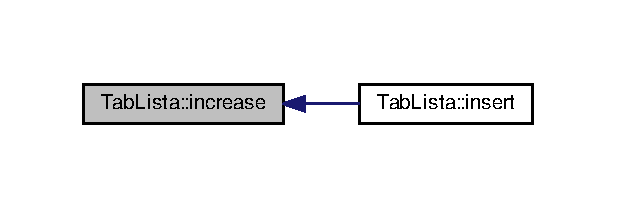
\includegraphics[width=296pt]{class_tab_lista_a9ae6a784d488c8b9885ccbc945225f9e_icgraph}
\end{center}
\end{figure}


\hypertarget{class_tab_lista_a7bd3e5f62a81bfd3813ad874e8a9c059}{\index{Tab\-Lista@{Tab\-Lista}!insert@{insert}}
\index{insert@{insert}!TabLista@{Tab\-Lista}}
\subsubsection[{insert}]{\setlength{\rightskip}{0pt plus 5cm}void Tab\-Lista\-::insert (
\begin{DoxyParamCaption}
\item[{int}]{\-\_\-elem}
\end{DoxyParamCaption}
)}}\label{class_tab_lista_a7bd3e5f62a81bfd3813ad874e8a9c059}

\begin{DoxyParams}[1]{Parametry}
\mbox{\tt in}  & {\em \-\_\-elem} & -\/ dodawany element. \\
\hline
\end{DoxyParams}


Definicja w linii 44 pliku tab\-\_\-lista.\-cpp.



Oto graf wywołań dla tej funkcji\-:\nopagebreak
\begin{figure}[H]
\begin{center}
\leavevmode
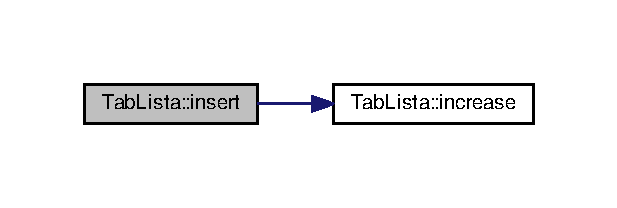
\includegraphics[width=296pt]{class_tab_lista_a7bd3e5f62a81bfd3813ad874e8a9c059_cgraph}
\end{center}
\end{figure}


\hypertarget{class_tab_lista_aae59a3eafbbd7424a952badb26410a5e}{\index{Tab\-Lista@{Tab\-Lista}!remove@{remove}}
\index{remove@{remove}!TabLista@{Tab\-Lista}}
\subsubsection[{remove}]{\setlength{\rightskip}{0pt plus 5cm}int Tab\-Lista\-::remove (
\begin{DoxyParamCaption}
\item[{int}]{\-\_\-f}
\end{DoxyParamCaption}
)}}\label{class_tab_lista_aae59a3eafbbd7424a952badb26410a5e}

\begin{DoxyParams}[1]{Parametry}
\mbox{\tt in}  & {\em \-\_\-f} & -\/ indeks elementu do usuniecia. \\
\hline
\end{DoxyParams}
\begin{DoxyReturn}{Zwraca}
-\/ usuwany element. 
\end{DoxyReturn}


Definicja w linii 53 pliku tab\-\_\-lista.\-cpp.



\subsection{Dokumentacja atrybutów składowych}
\hypertarget{class_tab_lista_ac7413a3d41c2c2e57fa92e055fc2e5b3}{\index{Tab\-Lista@{Tab\-Lista}!last@{last}}
\index{last@{last}!TabLista@{Tab\-Lista}}
\subsubsection[{last}]{\setlength{\rightskip}{0pt plus 5cm}long Tab\-Lista\-::last\hspace{0.3cm}{\ttfamily [private]}}}\label{class_tab_lista_ac7413a3d41c2c2e57fa92e055fc2e5b3}


Definicja w linii 23 pliku tab\-\_\-lista.\-hh.

\hypertarget{class_tab_lista_aa3c6d623be318ec8410fa447281380da}{\index{Tab\-Lista@{Tab\-Lista}!size@{size}}
\index{size@{size}!TabLista@{Tab\-Lista}}
\subsubsection[{size}]{\setlength{\rightskip}{0pt plus 5cm}long Tab\-Lista\-::size\hspace{0.3cm}{\ttfamily [private]}}}\label{class_tab_lista_aa3c6d623be318ec8410fa447281380da}


Definicja w linii 19 pliku tab\-\_\-lista.\-hh.

\hypertarget{class_tab_lista_a06f658ed62f3db852813e90dcc5876a5}{\index{Tab\-Lista@{Tab\-Lista}!tab@{tab}}
\index{tab@{tab}!TabLista@{Tab\-Lista}}
\subsubsection[{tab}]{\setlength{\rightskip}{0pt plus 5cm}int$\ast$ Tab\-Lista\-::tab\hspace{0.3cm}{\ttfamily [private]}}}\label{class_tab_lista_a06f658ed62f3db852813e90dcc5876a5}


Definicja w linii 15 pliku tab\-\_\-lista.\-hh.



Dokumentacja dla tej klasy została wygenerowana z plików\-:\begin{DoxyCompactItemize}
\item 
\hyperlink{tab__lista_8hh}{tab\-\_\-lista.\-hh}\item 
\hyperlink{tab__lista_8cpp}{tab\-\_\-lista.\-cpp}\end{DoxyCompactItemize}

\chapter{Dokumentacja plików}
\hypertarget{algorithm2_8cpp}{\section{Dokumentacja pliku algorithm2.\-cpp}
\label{algorithm2_8cpp}\index{algorithm2.\-cpp@{algorithm2.\-cpp}}
}
{\ttfamily \#include $<$iostream$>$}\\*
{\ttfamily \#include \char`\"{}stos.\-hh\char`\"{}}\\*
{\ttfamily \#include \char`\"{}benchmark.\-hh\char`\"{}}\\*
{\ttfamily \#include \char`\"{}algorithm2.\-hh\char`\"{}}\\*
Wykres zależności załączania dla algorithm2.\-cpp\-:\nopagebreak
\begin{figure}[H]
\begin{center}
\leavevmode
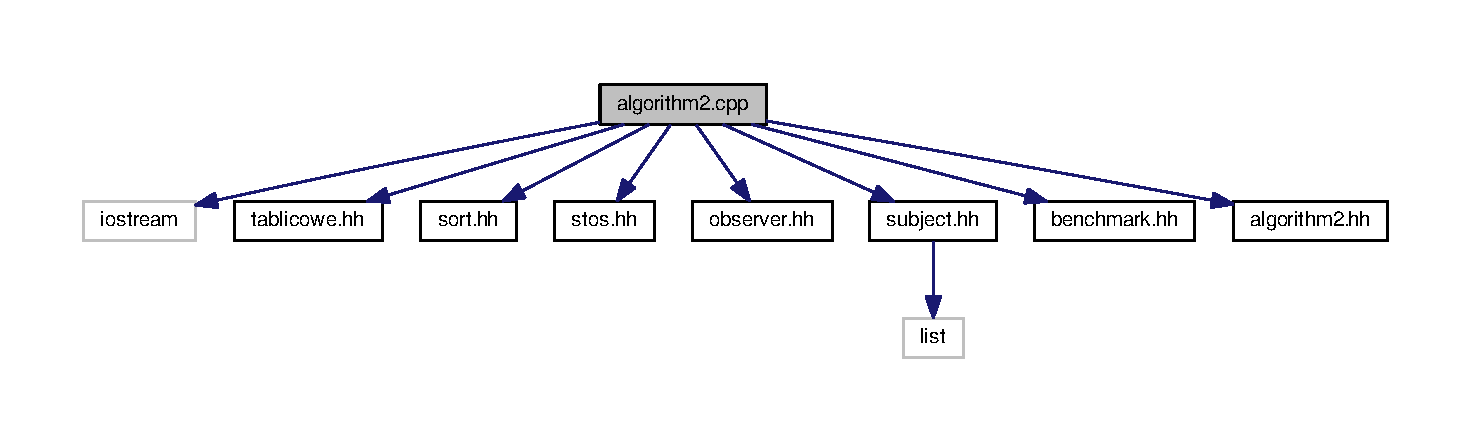
\includegraphics[width=350pt]{algorithm2_8cpp__incl}
\end{center}
\end{figure}

\hypertarget{algorithm2_8hh}{\section{Dokumentacja pliku algorithm2.\-hh}
\label{algorithm2_8hh}\index{algorithm2.\-hh@{algorithm2.\-hh}}
}
Ten wykres pokazuje, które pliki bezpośrednio lub pośrednio załączają ten plik\-:\nopagebreak
\begin{figure}[H]
\begin{center}
\leavevmode
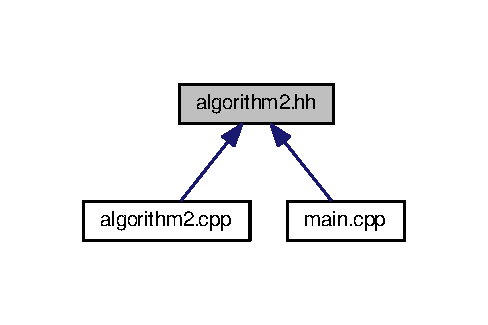
\includegraphics[width=234pt]{algorithm2_8hh__dep__incl}
\end{center}
\end{figure}
\subsection*{Komponenty}
\begin{DoxyCompactItemize}
\item 
class \hyperlink{class_algorithm2}{Algorithm2}
\begin{DoxyCompactList}\small\item\em Klasa \hyperlink{class_algorithm2}{Algorithm2} modelujaca algorytm sortowania stosu. Obiekt tego typu reprezentuje algorytm wykonujacy sortowanie szybkie na elementach stosu. Dziedziczy po klasie \hyperlink{class_benchmark}{Benchmark}. \end{DoxyCompactList}\end{DoxyCompactItemize}

\hypertarget{algorithm__kolejka_8cpp}{\section{Dokumentacja pliku algorithm\-\_\-kolejka.\-cpp}
\label{algorithm__kolejka_8cpp}\index{algorithm\-\_\-kolejka.\-cpp@{algorithm\-\_\-kolejka.\-cpp}}
}
{\ttfamily \#include $<$iostream$>$}\\*
{\ttfamily \#include \char`\"{}kolejka.\-hh\char`\"{}}\\*
{\ttfamily \#include \char`\"{}benchmark.\-hh\char`\"{}}\\*
{\ttfamily \#include \char`\"{}algorithm\-\_\-kolejka.\-hh\char`\"{}}\\*
Wykres zależności załączania dla algorithm\-\_\-kolejka.\-cpp\-:\nopagebreak
\begin{figure}[H]
\begin{center}
\leavevmode
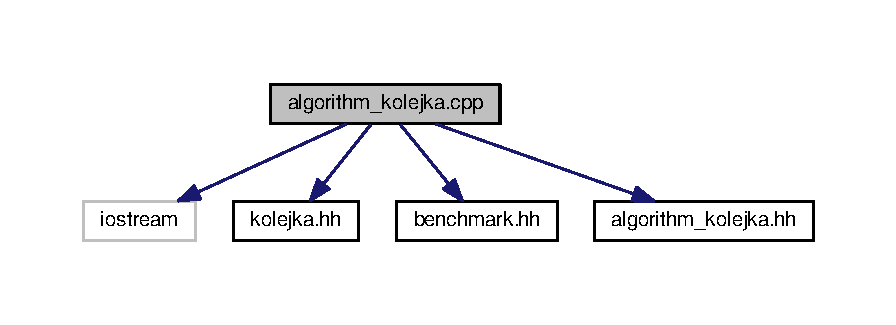
\includegraphics[width=350pt]{algorithm__kolejka_8cpp__incl}
\end{center}
\end{figure}

\hypertarget{algorithm__kolejka_8hh}{\section{Dokumentacja pliku algorithm\-\_\-kolejka.\-hh}
\label{algorithm__kolejka_8hh}\index{algorithm\-\_\-kolejka.\-hh@{algorithm\-\_\-kolejka.\-hh}}
}
Ten wykres pokazuje, które pliki bezpośrednio lub pośrednio załączają ten plik\-:\nopagebreak
\begin{figure}[H]
\begin{center}
\leavevmode
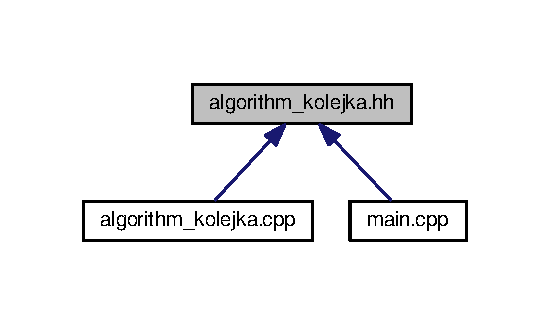
\includegraphics[width=264pt]{algorithm__kolejka_8hh__dep__incl}
\end{center}
\end{figure}
\subsection*{Komponenty}
\begin{DoxyCompactItemize}
\item 
class \hyperlink{class_algorithm_kolejka}{Algorithm\-Kolejka}
\begin{DoxyCompactList}\small\item\em Klasa \hyperlink{class_algorithm_kolejka}{Algorithm\-Kolejka} modelujaca algorytm wczytywania do kolejki. Obiekt tego typu reprezentuje algorytm wykonujacy wykonujacy wczytywanie zadanej ilosci elementow do kolejki. \end{DoxyCompactList}\end{DoxyCompactItemize}

\hypertarget{algorithm__lista_8cpp}{\section{Dokumentacja pliku algorithm\-\_\-lista.\-cpp}
\label{algorithm__lista_8cpp}\index{algorithm\-\_\-lista.\-cpp@{algorithm\-\_\-lista.\-cpp}}
}
{\ttfamily \#include $<$iostream$>$}\\*
{\ttfamily \#include \char`\"{}lista.\-hh\char`\"{}}\\*
{\ttfamily \#include \char`\"{}benchmark.\-hh\char`\"{}}\\*
{\ttfamily \#include \char`\"{}algorithm\-\_\-lista.\-hh\char`\"{}}\\*
Wykres zależności załączania dla algorithm\-\_\-lista.\-cpp\-:\nopagebreak
\begin{figure}[H]
\begin{center}
\leavevmode
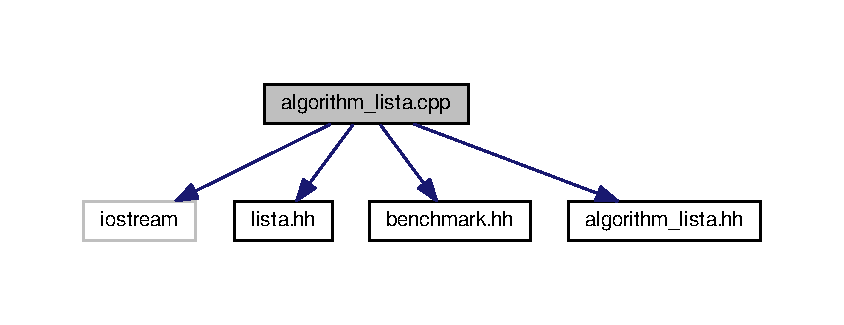
\includegraphics[width=350pt]{algorithm__lista_8cpp__incl}
\end{center}
\end{figure}

\hypertarget{algorithm__lista_8hh}{\section{Dokumentacja pliku algorithm\-\_\-lista.\-hh}
\label{algorithm__lista_8hh}\index{algorithm\-\_\-lista.\-hh@{algorithm\-\_\-lista.\-hh}}
}
Ten wykres pokazuje, które pliki bezpośrednio lub pośrednio załączają ten plik\-:\nopagebreak
\begin{figure}[H]
\begin{center}
\leavevmode
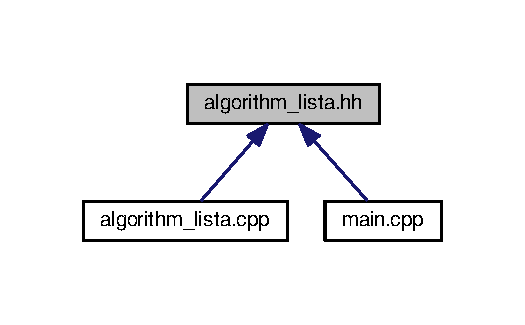
\includegraphics[width=252pt]{algorithm__lista_8hh__dep__incl}
\end{center}
\end{figure}
\subsection*{Komponenty}
\begin{DoxyCompactItemize}
\item 
class \hyperlink{class_algorithm_lista}{Algorithm\-Lista}
\begin{DoxyCompactList}\small\item\em Klasa \hyperlink{class_algorithm_lista}{Algorithm\-Lista} modelujaca algorytm wczytywania do kolejki. Obiekt tego typu reprezentuje algorytm wykonujacy wykonujacy wczytywanie zadanej ilosci elementow do listy. \end{DoxyCompactList}\end{DoxyCompactItemize}

\hypertarget{algorithm__stos_8cpp}{\section{Dokumentacja pliku algorithm\-\_\-stos.\-cpp}
\label{algorithm__stos_8cpp}\index{algorithm\-\_\-stos.\-cpp@{algorithm\-\_\-stos.\-cpp}}
}
{\ttfamily \#include $<$iostream$>$}\\*
{\ttfamily \#include \char`\"{}stos.\-hh\char`\"{}}\\*
{\ttfamily \#include \char`\"{}benchmark.\-hh\char`\"{}}\\*
{\ttfamily \#include \char`\"{}algorithm\-\_\-stos.\-hh\char`\"{}}\\*
Wykres zależności załączania dla algorithm\-\_\-stos.\-cpp\-:\nopagebreak
\begin{figure}[H]
\begin{center}
\leavevmode
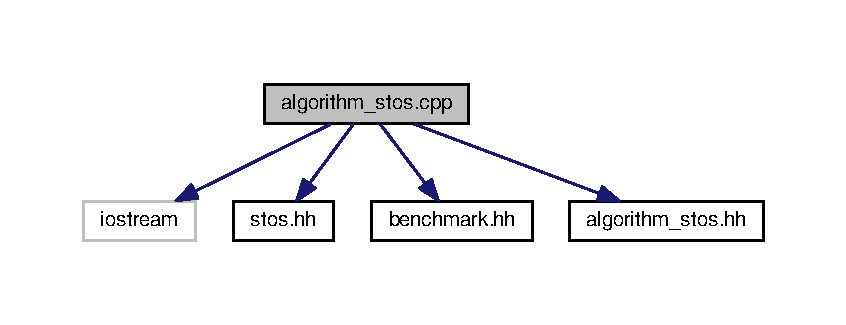
\includegraphics[width=350pt]{algorithm__stos_8cpp__incl}
\end{center}
\end{figure}

\hypertarget{algorithm__stos_8hh}{\section{Dokumentacja pliku algorithm\-\_\-stos.\-hh}
\label{algorithm__stos_8hh}\index{algorithm\-\_\-stos.\-hh@{algorithm\-\_\-stos.\-hh}}
}
Ten wykres pokazuje, które pliki bezpośrednio lub pośrednio załączają ten plik\-:\nopagebreak
\begin{figure}[H]
\begin{center}
\leavevmode
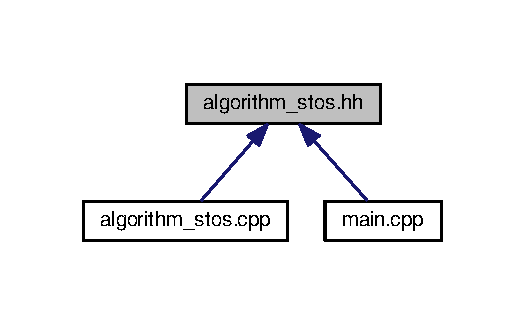
\includegraphics[width=252pt]{algorithm__stos_8hh__dep__incl}
\end{center}
\end{figure}
\subsection*{Komponenty}
\begin{DoxyCompactItemize}
\item 
class \hyperlink{class_algorithm_stos}{Algorithm\-Stos}
\begin{DoxyCompactList}\small\item\em Klasa \hyperlink{class_algorithm_stos}{Algorithm\-Stos} modelujaca algorytm wczytywania do stosu. Obiekt tego typu reprezentuje algorytm wykonujacy wykonujacy wczytywanie zadanej ilosci elementow do stosu. \end{DoxyCompactList}\end{DoxyCompactItemize}

\hypertarget{benchmark_8cpp}{\section{Dokumentacja pliku benchmark.\-cpp}
\label{benchmark_8cpp}\index{benchmark.\-cpp@{benchmark.\-cpp}}
}
{\ttfamily \#include $<$iostream$>$}\\*
{\ttfamily \#include $<$fstream$>$}\\*
{\ttfamily \#include $<$chrono$>$}\\*
{\ttfamily \#include \char`\"{}benchmark.\-hh\char`\"{}}\\*
Wykres zależności załączania dla benchmark.\-cpp\-:\nopagebreak
\begin{figure}[H]
\begin{center}
\leavevmode
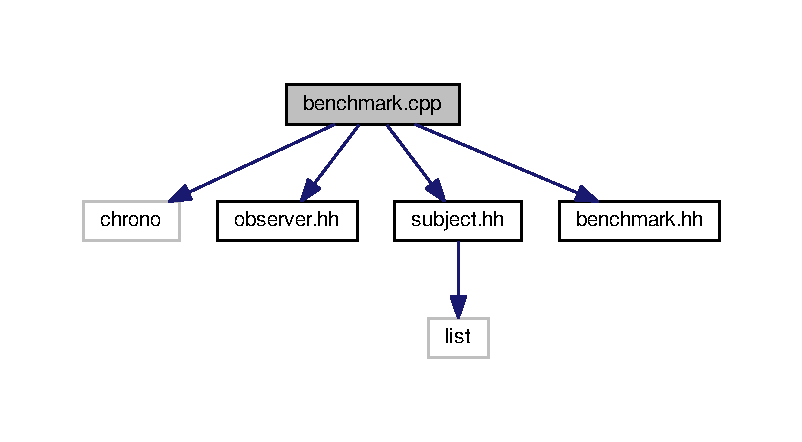
\includegraphics[width=350pt]{benchmark_8cpp__incl}
\end{center}
\end{figure}
\subsection*{Definicje}
\begin{DoxyCompactItemize}
\item 
\#define \hyperlink{benchmark_8cpp_a30362161c93e3f1a4ee4c673f535b5a8}{L\-E\-N\-G\-T\-H}~8
\item 
\#define \hyperlink{benchmark_8cpp_a96de703b1d261e201a5cbb65b4590f89}{R\-E\-P\-E\-A\-T\-S}~3
\end{DoxyCompactItemize}


\subsection{Dokumentacja definicji}
\hypertarget{benchmark_8cpp_a30362161c93e3f1a4ee4c673f535b5a8}{\index{benchmark.\-cpp@{benchmark.\-cpp}!L\-E\-N\-G\-T\-H@{L\-E\-N\-G\-T\-H}}
\index{L\-E\-N\-G\-T\-H@{L\-E\-N\-G\-T\-H}!benchmark.cpp@{benchmark.\-cpp}}
\subsubsection[{L\-E\-N\-G\-T\-H}]{\setlength{\rightskip}{0pt plus 5cm}\#define L\-E\-N\-G\-T\-H~8}}\label{benchmark_8cpp_a30362161c93e3f1a4ee4c673f535b5a8}


Definicja w linii 7 pliku benchmark.\-cpp.

\hypertarget{benchmark_8cpp_a96de703b1d261e201a5cbb65b4590f89}{\index{benchmark.\-cpp@{benchmark.\-cpp}!R\-E\-P\-E\-A\-T\-S@{R\-E\-P\-E\-A\-T\-S}}
\index{R\-E\-P\-E\-A\-T\-S@{R\-E\-P\-E\-A\-T\-S}!benchmark.cpp@{benchmark.\-cpp}}
\subsubsection[{R\-E\-P\-E\-A\-T\-S}]{\setlength{\rightskip}{0pt plus 5cm}\#define R\-E\-P\-E\-A\-T\-S~3}}\label{benchmark_8cpp_a96de703b1d261e201a5cbb65b4590f89}


Definicja w linii 8 pliku benchmark.\-cpp.


\hypertarget{benchmark_8hh}{\section{Dokumentacja pliku benchmark.\-hh}
\label{benchmark_8hh}\index{benchmark.\-hh@{benchmark.\-hh}}
}
Ten wykres pokazuje, które pliki bezpośrednio lub pośrednio załączają ten plik\-:\nopagebreak
\begin{figure}[H]
\begin{center}
\leavevmode
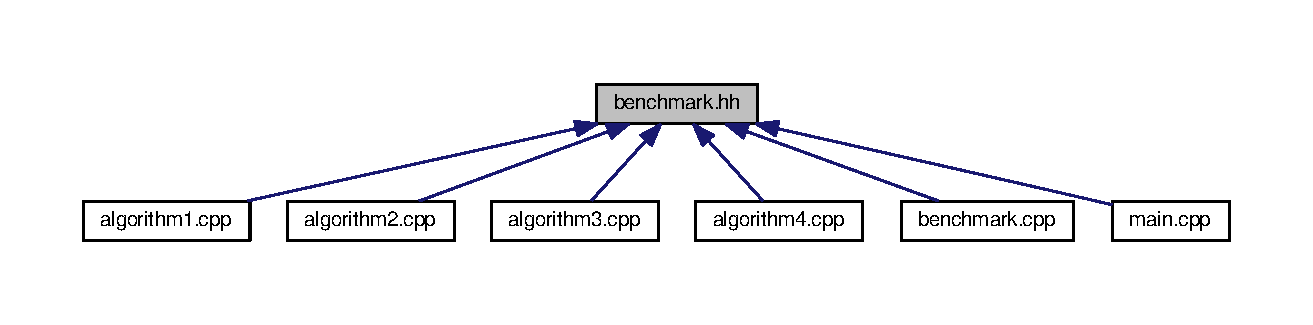
\includegraphics[width=350pt]{benchmark_8hh__dep__incl}
\end{center}
\end{figure}
\subsection*{Komponenty}
\begin{DoxyCompactItemize}
\item 
class \hyperlink{class_benchmark}{Benchmark}
\begin{DoxyCompactList}\small\item\em Klasa \hyperlink{class_benchmark}{Benchmark} modelujaca program benchmarkujacy. Obiekt tego typu reprezentuje program sprawdzajacy szybkosc wykonywania algorytmow. Dziedziczy po klasie \hyperlink{class_subject}{Subject}. \end{DoxyCompactList}\end{DoxyCompactItemize}
\subsection*{Definicje}
\begin{DoxyCompactItemize}
\item 
\#define \hyperlink{benchmark_8hh_a70ed59adcb4159ac551058053e649640}{S\-I\-Z\-E}~100000
\end{DoxyCompactItemize}


\subsection{Dokumentacja definicji}
\hypertarget{benchmark_8hh_a70ed59adcb4159ac551058053e649640}{\index{benchmark.\-hh@{benchmark.\-hh}!S\-I\-Z\-E@{S\-I\-Z\-E}}
\index{S\-I\-Z\-E@{S\-I\-Z\-E}!benchmark.hh@{benchmark.\-hh}}
\subsubsection[{S\-I\-Z\-E}]{\setlength{\rightskip}{0pt plus 5cm}\#define S\-I\-Z\-E~100000}}\label{benchmark_8hh_a70ed59adcb4159ac551058053e649640}


Definicja w linii 4 pliku benchmark.\-hh.


\hypertarget{generate_8cpp}{\section{Dokumentacja pliku generate.\-cpp}
\label{generate_8cpp}\index{generate.\-cpp@{generate.\-cpp}}
}
{\ttfamily \#include $<$fstream$>$}\\*
{\ttfamily \#include $<$iostream$>$}\\*
{\ttfamily \#include $<$cstdlib$>$}\\*
Wykres zależności załączania dla generate.\-cpp\-:\nopagebreak
\begin{figure}[H]
\begin{center}
\leavevmode
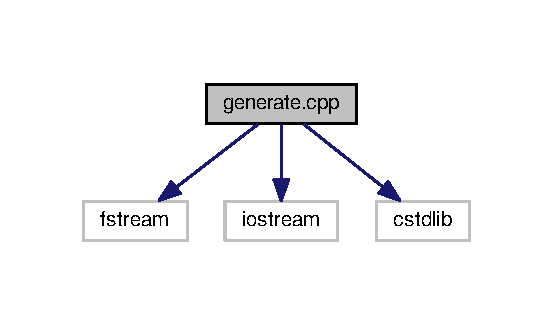
\includegraphics[width=265pt]{generate_8cpp__incl}
\end{center}
\end{figure}
\subsection*{Definicje}
\begin{DoxyCompactItemize}
\item 
\#define \hyperlink{generate_8cpp_a70ed59adcb4159ac551058053e649640}{S\-I\-Z\-E}~10000000
\end{DoxyCompactItemize}
\subsection*{Funkcje}
\begin{DoxyCompactItemize}
\item 
int \hyperlink{generate_8cpp_ae66f6b31b5ad750f1fe042a706a4e3d4}{main} ()
\begin{DoxyCompactList}\small\item\em Funkcja generowania pliku z danymi wejsciowymi. Generuje liczby losowe od 1 do 51 i zapisuje je do pliku o nazwie data.\-txt. \end{DoxyCompactList}\end{DoxyCompactItemize}


\subsection{Dokumentacja definicji}
\hypertarget{generate_8cpp_a70ed59adcb4159ac551058053e649640}{\index{generate.\-cpp@{generate.\-cpp}!S\-I\-Z\-E@{S\-I\-Z\-E}}
\index{S\-I\-Z\-E@{S\-I\-Z\-E}!generate.cpp@{generate.\-cpp}}
\subsubsection[{S\-I\-Z\-E}]{\setlength{\rightskip}{0pt plus 5cm}\#define S\-I\-Z\-E~10000000}}\label{generate_8cpp_a70ed59adcb4159ac551058053e649640}


Definicja w linii 5 pliku generate.\-cpp.



\subsection{Dokumentacja funkcji}
\hypertarget{generate_8cpp_ae66f6b31b5ad750f1fe042a706a4e3d4}{\index{generate.\-cpp@{generate.\-cpp}!main@{main}}
\index{main@{main}!generate.cpp@{generate.\-cpp}}
\subsubsection[{main}]{\setlength{\rightskip}{0pt plus 5cm}int main (
\begin{DoxyParamCaption}
{}
\end{DoxyParamCaption}
)}}\label{generate_8cpp_ae66f6b31b5ad750f1fe042a706a4e3d4}

\begin{DoxyRetVals}{Zwracane wartości}
{\em 0} & -\/ gdy funkcja zadziala poprawnie. \\
\hline
{\em 1} & -\/ gdy wystapi blad otwarcia pliku do zapisu. \\
\hline
\end{DoxyRetVals}


Definicja w linii 14 pliku generate.\-cpp.


\hypertarget{kolejka_8cpp}{\section{Dokumentacja pliku kolejka.\-cpp}
\label{kolejka_8cpp}\index{kolejka.\-cpp@{kolejka.\-cpp}}
}
{\ttfamily \#include $<$iostream$>$}\\*
{\ttfamily \#include \char`\"{}tablicowe.\-hh\char`\"{}}\\*
{\ttfamily \#include \char`\"{}kolejka.\-hh\char`\"{}}\\*
Wykres zależności załączania dla kolejka.\-cpp\-:
\nopagebreak
\begin{figure}[H]
\begin{center}
\leavevmode
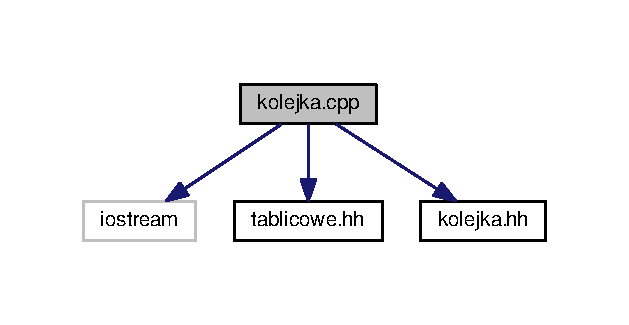
\includegraphics[width=302pt]{kolejka_8cpp__incl}
\end{center}
\end{figure}

\hypertarget{kolejka_8hh}{\section{Dokumentacja pliku kolejka.\-hh}
\label{kolejka_8hh}\index{kolejka.\-hh@{kolejka.\-hh}}
}
Ten wykres pokazuje, które pliki bezpośrednio lub pośrednio załączają ten plik\-:
\nopagebreak
\begin{figure}[H]
\begin{center}
\leavevmode
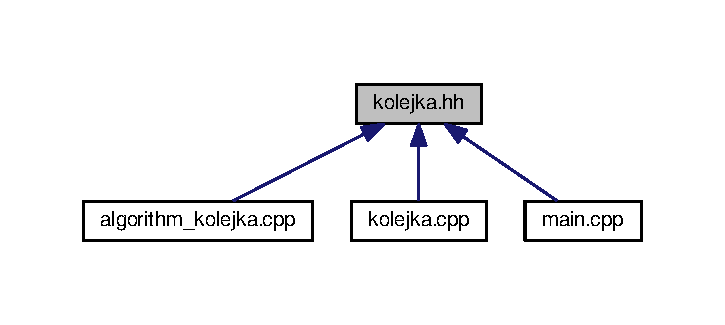
\includegraphics[width=219pt]{kolejka_8hh__dep__incl}
\end{center}
\end{figure}
\subsection*{Komponenty}
\begin{DoxyCompactItemize}
\item 
class \hyperlink{class_kolejka}{Kolejka}
\begin{DoxyCompactList}\small\item\em Klasa \hyperlink{class_kolejka}{Kolejka} modelujaca strukture danych typu kolejka. Obiekt tego typu reprezentuje strukture danych typu kolejka wraz z operacjami mozliwymi do wykonania na tej strukturze. Dziedziczy po klasie \hyperlink{class_tablicowe}{Tablicowe}. \end{DoxyCompactList}\end{DoxyCompactItemize}

\hypertarget{lista_8cpp}{\section{Dokumentacja pliku lista.\-cpp}
\label{lista_8cpp}\index{lista.\-cpp@{lista.\-cpp}}
}
{\ttfamily \#include $<$iostream$>$}\\*
{\ttfamily \#include \char`\"{}lista.\-hh\char`\"{}}\\*
Wykres zależności załączania dla lista.\-cpp\-:
\nopagebreak
\begin{figure}[H]
\begin{center}
\leavevmode
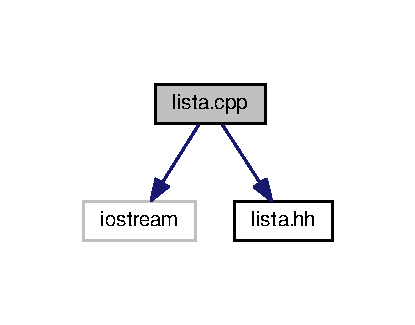
\includegraphics[width=199pt]{lista_8cpp__incl}
\end{center}
\end{figure}

\hypertarget{lista_8hh}{\section{Dokumentacja pliku lista.\-hh}
\label{lista_8hh}\index{lista.\-hh@{lista.\-hh}}
}
Ten wykres pokazuje, które pliki bezpośrednio lub pośrednio załączają ten plik\-:\nopagebreak
\begin{figure}[H]
\begin{center}
\leavevmode
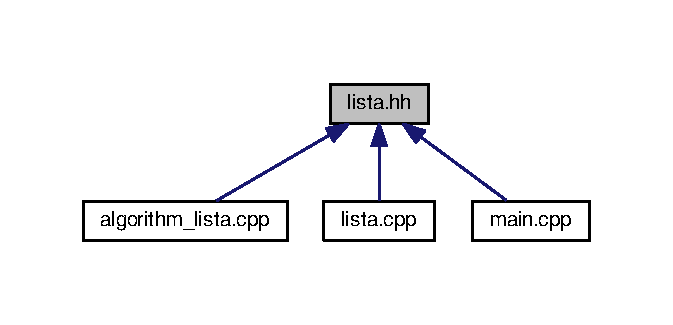
\includegraphics[width=207pt]{lista_8hh__dep__incl}
\end{center}
\end{figure}
\subsection*{Komponenty}
\begin{DoxyCompactItemize}
\item 
struct \hyperlink{struct_komorka}{Komorka}
\begin{DoxyCompactList}\small\item\em Struktura \hyperlink{struct_komorka}{Komorka}. Obiekt tego typu reprezentuje pojedyncza komorke wraz ze wskaznikiem na nastepna komorke listy. \end{DoxyCompactList}\item 
struct \hyperlink{struct_lista}{Lista}
\begin{DoxyCompactList}\small\item\em Klasa \hyperlink{struct_lista}{Lista} modelujaca strukture danych typu lista. Obiekt tego typu reprezentuje strukture danych typu lista wraz z operacjami mozliwymi do wykonania na tej strukturze. \end{DoxyCompactList}\end{DoxyCompactItemize}

\hypertarget{main_8cpp}{\section{Dokumentacja pliku main.\-cpp}
\label{main_8cpp}\index{main.\-cpp@{main.\-cpp}}
}
{\ttfamily \#include $<$iostream$>$}\\*
{\ttfamily \#include \char`\"{}observer.\-hh\char`\"{}}\\*
{\ttfamily \#include \char`\"{}subject.\-hh\char`\"{}}\\*
{\ttfamily \#include \char`\"{}benchmark.\-hh\char`\"{}}\\*
{\ttfamily \#include \char`\"{}writing\-\_\-observer.\-hh\char`\"{}}\\*
{\ttfamily \#include \char`\"{}tablicowe.\-hh\char`\"{}}\\*
{\ttfamily \#include \char`\"{}sort.\-hh\char`\"{}}\\*
{\ttfamily \#include \char`\"{}stos.\-hh\char`\"{}}\\*
{\ttfamily \#include \char`\"{}kolejka.\-hh\char`\"{}}\\*
{\ttfamily \#include \char`\"{}lista.\-hh\char`\"{}}\\*
{\ttfamily \#include \char`\"{}tab\-\_\-lista.\-hh\char`\"{}}\\*
{\ttfamily \#include \char`\"{}asocjacyjna.\-hh\char`\"{}}\\*
{\ttfamily \#include \char`\"{}mieszajaca.\-hh\char`\"{}}\\*
{\ttfamily \#include \char`\"{}binary\-\_\-tree.\-hh\char`\"{}}\\*
{\ttfamily \#include \char`\"{}rb\-\_\-tree.\-hh\char`\"{}}\\*
{\ttfamily \#include \char`\"{}algorithm1.\-hh\char`\"{}}\\*
{\ttfamily \#include \char`\"{}algorithm2.\-hh\char`\"{}}\\*
{\ttfamily \#include \char`\"{}algorithm3.\-hh\char`\"{}}\\*
{\ttfamily \#include \char`\"{}algorithm4.\-hh\char`\"{}}\\*
Wykres zależności załączania dla main.\-cpp\-:
\nopagebreak
\begin{figure}[H]
\begin{center}
\leavevmode
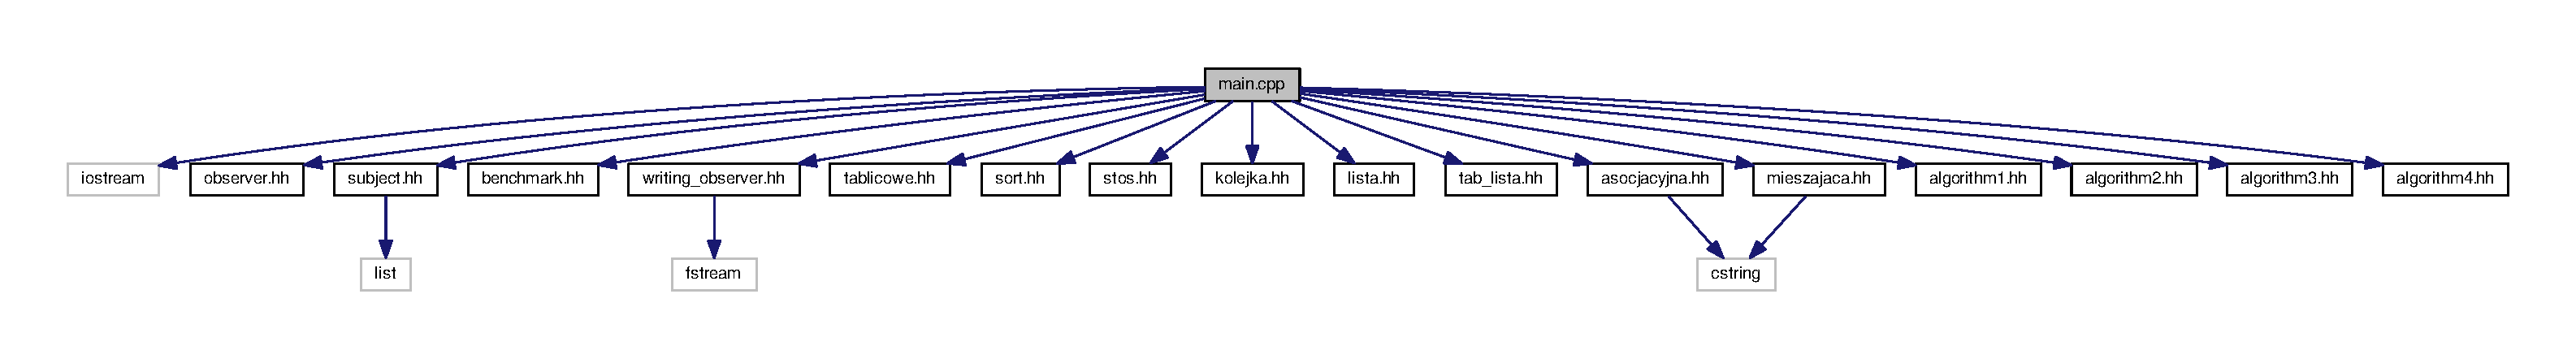
\includegraphics[width=350pt]{main_8cpp__incl}
\end{center}
\end{figure}
\subsection*{Funkcje}
\begin{DoxyCompactItemize}
\item 
int \hyperlink{main_8cpp_ae66f6b31b5ad750f1fe042a706a4e3d4}{main} ()
\begin{DoxyCompactList}\small\item\em Funkcja tworzaca i testujaca algorytm. Wczytuje dane otrzymane na strumien wejsciowy do tablicy data\mbox{[}\mbox{]}. Nastepnie tworzy obiekt \hyperlink{class_benchmark}{Benchmark} oraz obiekt Potegowanie. Pozniej uruchamia metode testujaca w obiekcie klasy \hyperlink{class_benchmark}{Benchmark} dla obiektu klasy Potegowanie. \end{DoxyCompactList}\end{DoxyCompactItemize}


\subsection{Dokumentacja funkcji}
\hypertarget{main_8cpp_ae66f6b31b5ad750f1fe042a706a4e3d4}{\index{main.\-cpp@{main.\-cpp}!main@{main}}
\index{main@{main}!main.cpp@{main.\-cpp}}
\subsubsection[{main}]{\setlength{\rightskip}{0pt plus 5cm}int main (
\begin{DoxyParamCaption}
{}
\end{DoxyParamCaption}
)}}\label{main_8cpp_ae66f6b31b5ad750f1fe042a706a4e3d4}

\begin{DoxyRetVals}{Zwracane wartości}
{\em 0} & -\/ domyslna wartosc zwracana przez funkcje. \\
\hline
\end{DoxyRetVals}


Definicja w linii 30 pliku main.\-cpp.


\hypertarget{stos_8cpp}{\section{Dokumentacja pliku stos.\-cpp}
\label{stos_8cpp}\index{stos.\-cpp@{stos.\-cpp}}
}
{\ttfamily \#include $<$iostream$>$}\\*
{\ttfamily \#include $<$cstdlib$>$}\\*
{\ttfamily \#include \char`\"{}stos.\-hh\char`\"{}}\\*
Wykres zależności załączania dla stos.\-cpp\-:\nopagebreak
\begin{figure}[H]
\begin{center}
\leavevmode
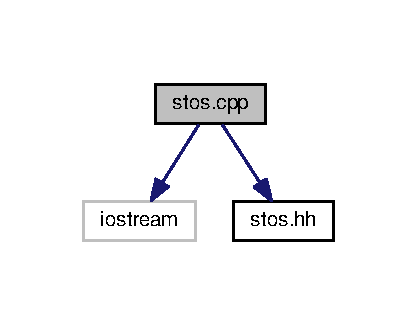
\includegraphics[width=264pt]{stos_8cpp__incl}
\end{center}
\end{figure}

\hypertarget{stos_8hh}{\section{Dokumentacja pliku stos.\-hh}
\label{stos_8hh}\index{stos.\-hh@{stos.\-hh}}
}
Ten wykres pokazuje, które pliki bezpośrednio lub pośrednio załączają ten plik\-:
\nopagebreak
\begin{figure}[H]
\begin{center}
\leavevmode
\includegraphics[width=207pt]{stos_8hh__dep__incl}
\end{center}
\end{figure}
\subsection*{Komponenty}
\begin{DoxyCompactItemize}
\item 
struct \hyperlink{struct_stos}{Stos}
\begin{DoxyCompactList}\small\item\em Klasa \hyperlink{struct_stos}{Stos} modelujaca strukture danych typu stos. Obiekt tego typu reprezentuje strukture danych typu stos wraz z operacjami mozliwymi do wykonania na tej strukturze. Dziedziczy po klasie \hyperlink{class_tablicowe}{Tablicowe}. \end{DoxyCompactList}\end{DoxyCompactItemize}

\hypertarget{strona-glowna_8dox}{\section{Dokumentacja pliku strona-\/glowna.dox}
\label{strona-glowna_8dox}\index{strona-\/glowna.\-dox@{strona-\/glowna.\-dox}}
}

\hypertarget{tab__lista_8cpp}{\section{Dokumentacja pliku tab\-\_\-lista.\-cpp}
\label{tab__lista_8cpp}\index{tab\-\_\-lista.\-cpp@{tab\-\_\-lista.\-cpp}}
}
{\ttfamily \#include $<$iostream$>$}\\*
{\ttfamily \#include \char`\"{}tab\-\_\-lista.\-hh\char`\"{}}\\*
Wykres zależności załączania dla tab\-\_\-lista.\-cpp\-:\nopagebreak
\begin{figure}[H]
\begin{center}
\leavevmode
\includegraphics[width=218pt]{tab__lista_8cpp__incl}
\end{center}
\end{figure}

\hypertarget{tab__lista_8hh}{\section{Dokumentacja pliku tab\-\_\-lista.\-hh}
\label{tab__lista_8hh}\index{tab\-\_\-lista.\-hh@{tab\-\_\-lista.\-hh}}
}
Ten wykres pokazuje, które pliki bezpośrednio lub pośrednio załączają ten plik\-:\nopagebreak
\begin{figure}[H]
\begin{center}
\leavevmode
\includegraphics[width=225pt]{tab__lista_8hh__dep__incl}
\end{center}
\end{figure}
\subsection*{Komponenty}
\begin{DoxyCompactItemize}
\item 
struct \hyperlink{struct_tab_lista}{Tab\-Lista}
\begin{DoxyCompactList}\small\item\em Klasa \hyperlink{struct_tab_lista}{Tab\-Lista} modelujaca strukture danych typu lista. Obiekt tego typu reprezentuje strukture danych typu lista zaimplementowana na tablicy dynamicznej. Obiekt zawiera rowniez podstowe metody listy. Dziedziczy po klasie \hyperlink{class_tablicowe}{Tablicowe}. \end{DoxyCompactList}\end{DoxyCompactItemize}

%--- End generated contents ---

% Index
\newpage
\phantomsection
\addcontentsline{toc}{chapter}{Indeks}
\printindex

\end{document}
